% !TeX program = xelatex

\documentclass[aspectratio=169]{beamer}
\usepackage{minted}
\usepackage{xcolor}
\usepackage{tcolorbox}
\usepackage{graphicx}
\usepackage{fontspec}
\usepackage{tabularray}

\usetheme{cexa-kokkos}

%\BeforeBeginEnvironment{minted}{\begin{tcolorbox}}
%\AfterEndEnvironment{minted}{\end{tcolorbox}}

\AtBeginSection{
    \begin{frame}{Outline}
        \tableofcontents[currentsection, hideothersubsections]
    \end{frame}
}

\AtBeginSubsection{
    \begin{frame}{Outline}
        \tableofcontents[currentsection, currentsubsection]
    \end{frame}
}

\setminted{
    autogobble,
    fontsize=\small,
    bgcolor=lightgray,
    xleftmargin=0.5em,
    xrightmargin=0.5em,
    breaklines,
}

\NewTblrTheme{kokkostable}{
    \SetTblrInner{
        width=\linewidth,
        rowhead=1,
        rows={ht=\baselineskip},
        row{odd}={bg=lightgray},
        row{1}={bg=lightmain},
    }
}

\graphicspath{{../../images/}}

%Information to be included in the title page:
\title[Kokkos and performance portability]{Kokkos and performance portability:\\an introduction for all}
\author{Mathieu Lobet and the CExA team}
\institute{CEA}
\date{2024}
\titlegraphic{%
    
\includegraphics[height=4em]{kokkos.png}%
    \hspace{1em}%
    
\includegraphics[height=4em]{cexa_logo.png}
}

% _____________________________________________________________________________

\begin{document}

\begin{frame}[plain]
    \titlepage
\end{frame}

% _____________________________________________________________________________

\begin{frame}{This course is open source}
    \begin{center}
        \githublink{\url{https://github.com/CExA-project/cexa-kokkos-tutorials}}
    \end{center}
\end{frame}

% _____________________________________________________________________________

\begin{frame}{Prerequisites}
    This course is intended for beginners in Kokkos and performance portability, without strong C++ knowledge

    \vspace{1em}

    \begin{block}{What you still need}
        \begin{itemize}
            \item Basic knowledge of C/C++
            \item Basic knowledge of parallel programming
            \item Basic knowledge of CMake
            \item Basic knowledge of a Linux environment
        \end{itemize}
    \end{block}
\end{frame}

% _____________________________________________________________________________

\begin{frame}{Schedule of the training}
    \begin{description}[Wednesday 15\textsuperscript{th} 15:30 -- 16:30]
        \item[Wednesday 15\textsuperscript{th} 15:30 -- 16:30] Introduction
        \item[Thursday 16\textsuperscript{th} 10:00 -- 17:00] Course and hands-on
        \item[Friday 17\textsuperscript{th} 09:00 -- 12:00] Hands-on and introduction to advanced features
    \end{description}
\end{frame}

\begin{frame}{Outline}
    \tableofcontents[hidesubsections]
\end{frame}

% _____________________________________________________________________________

\section{Introduction}

% _____________________________________________________________________________

\begin{frame}{Current supercomputers hardware}
    \begin{center}
        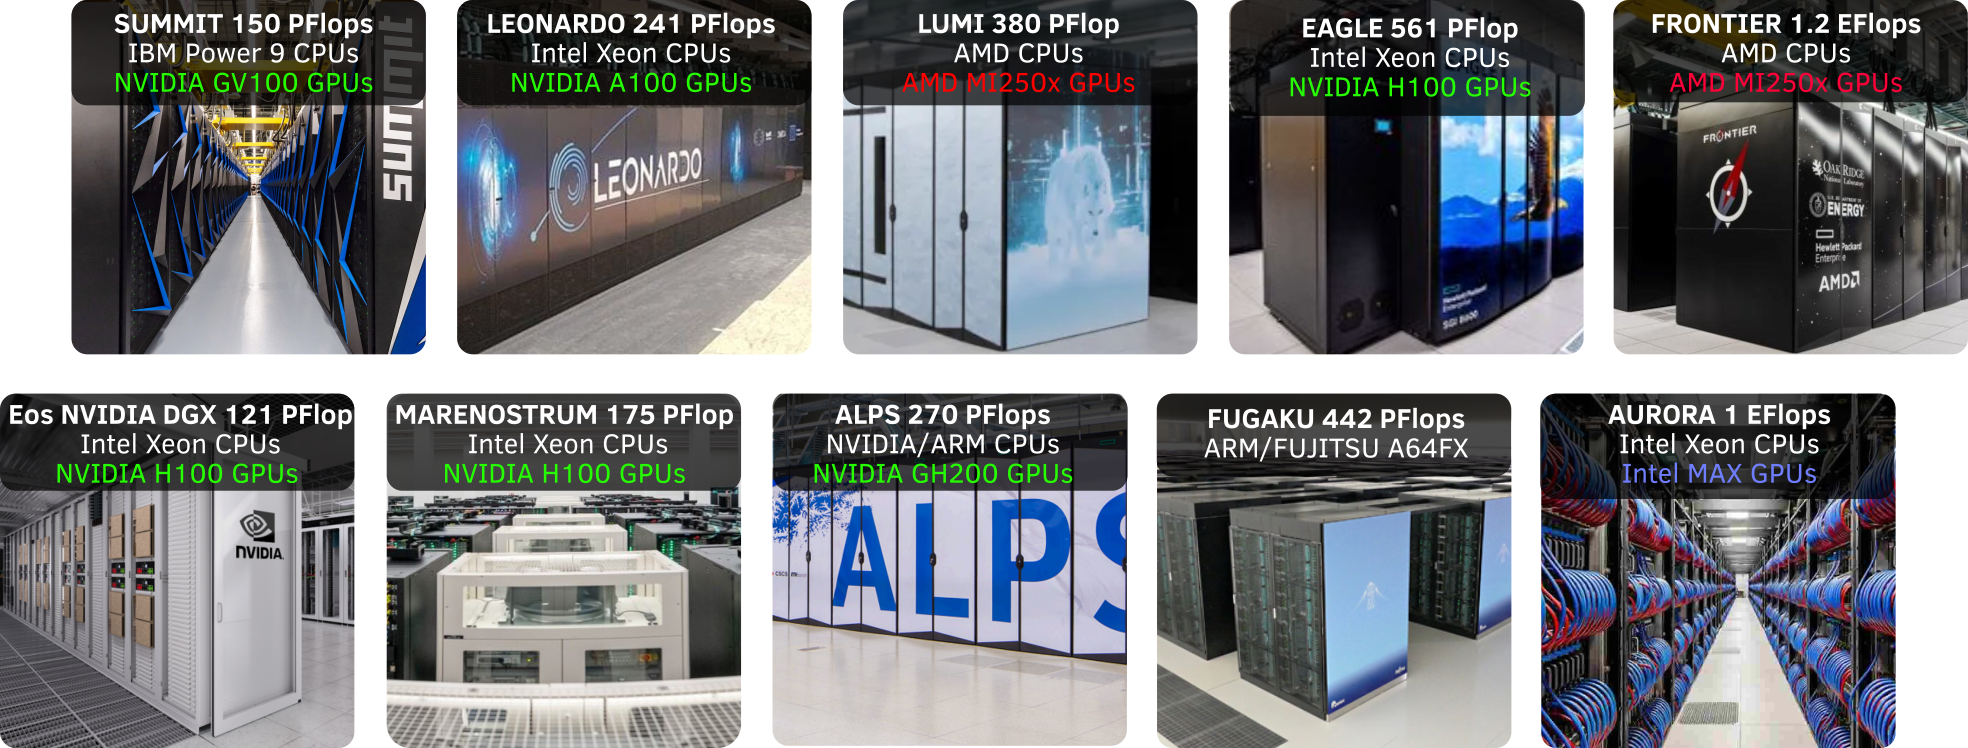
\includegraphics[width=0.8\textwidth]{top10_super_computers.png}

        \caption{Top 10 supercomputers in the world in June 2024}
    \end{center}
    \begin{itemize}
        \item Heterogeneous nodes: mix of CPU and GPU accelerators
        \item Many CPU (Intel, AMD, ARM, RISC) and GPU vendors (NVIDIA, AMD, Intel)
    \end{itemize}
\end{frame}

% _____________________________________________________________________________

\begin{frame}{EuroHPC supercomputers hardware}
    \begin{center}
        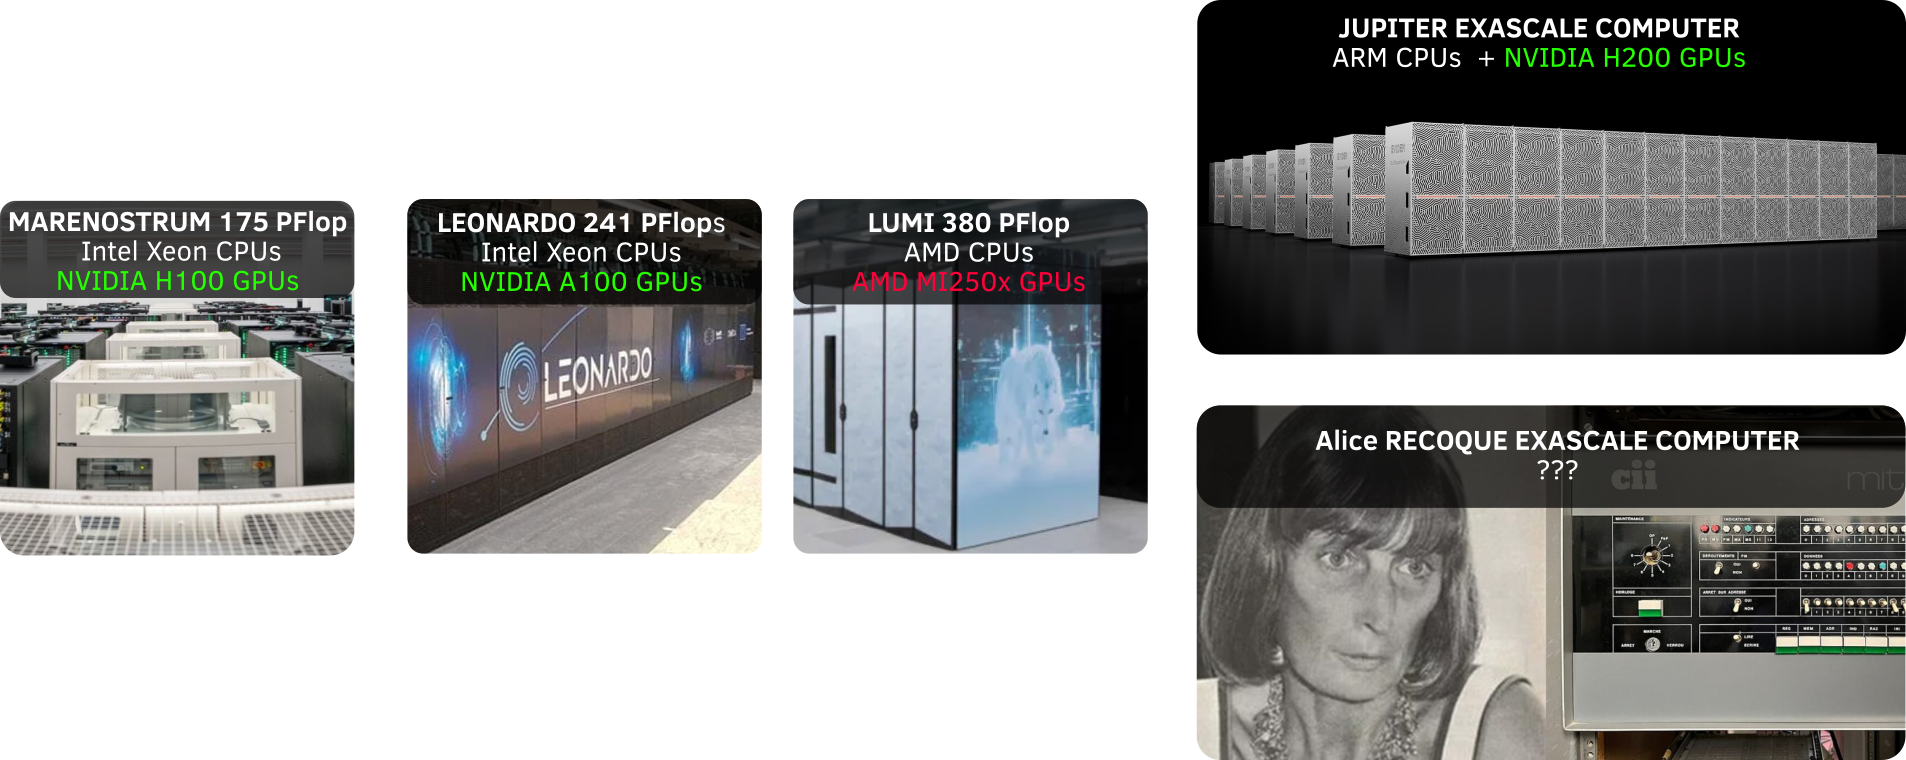
\includegraphics[width=1\textwidth]{euroHPC.png}

        \caption{EuroHPC supercomputers}
    \end{center}
\end{frame}

% _____________________________________________________________________________

\begin{frame}{Basic definition of a supercomputer}
    \begin{center}
        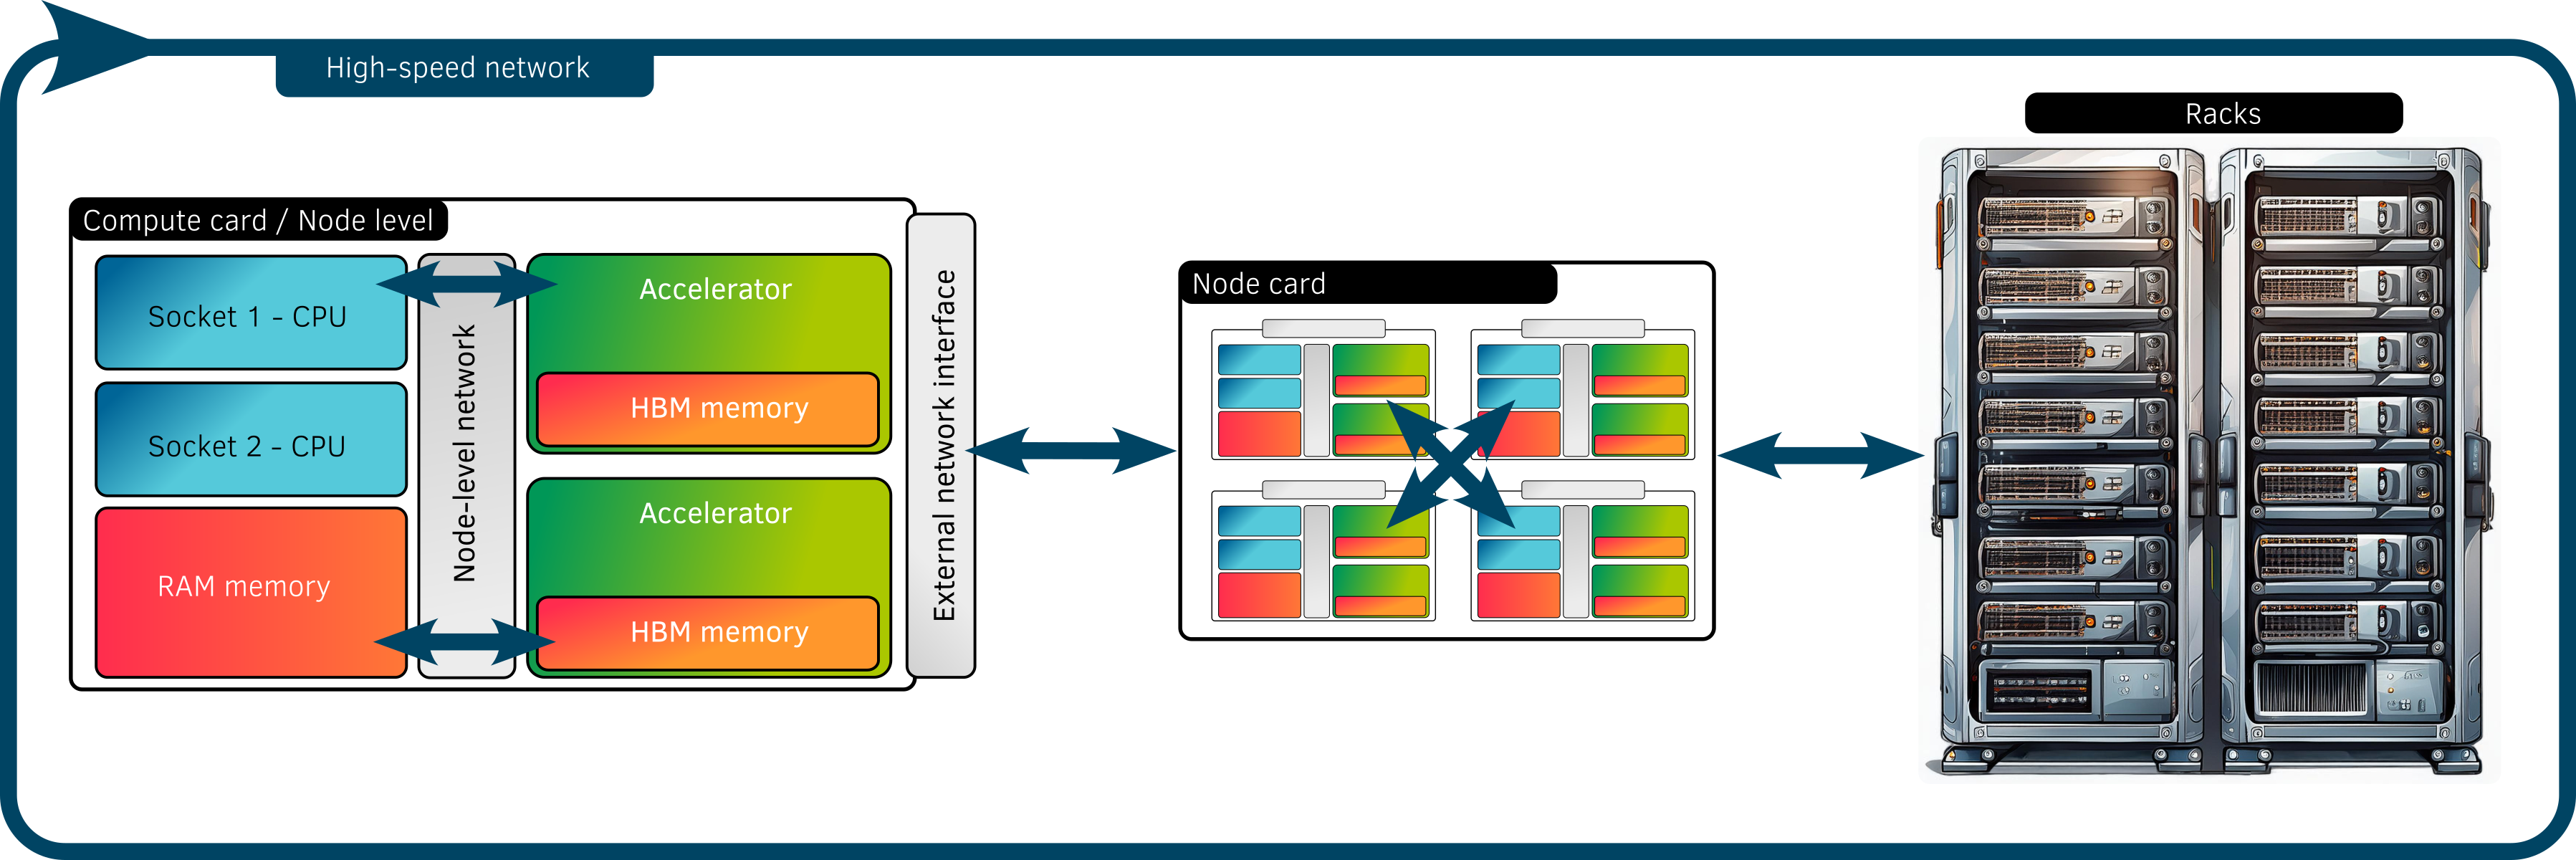
\includegraphics[width=0.8\textwidth]{super-computer_architecture.png}
    \end{center}
    \begin{itemize}
        \item Distributed memory system composed of many compute nodes packed into racks and linked by a high-speed network
        \item Compute nodes are composed of one or more CPUs and one or more accelerators
        \item Most common accelerators today are GPUs (aka GPGPU)
    \end{itemize}
\end{frame}

% _____________________________________________________________________________

\begin{frame}{Zoom on the CPU architecture}
    \begin{columns}
        \begin{column}{0.5\linewidth}
            \begin{center}
                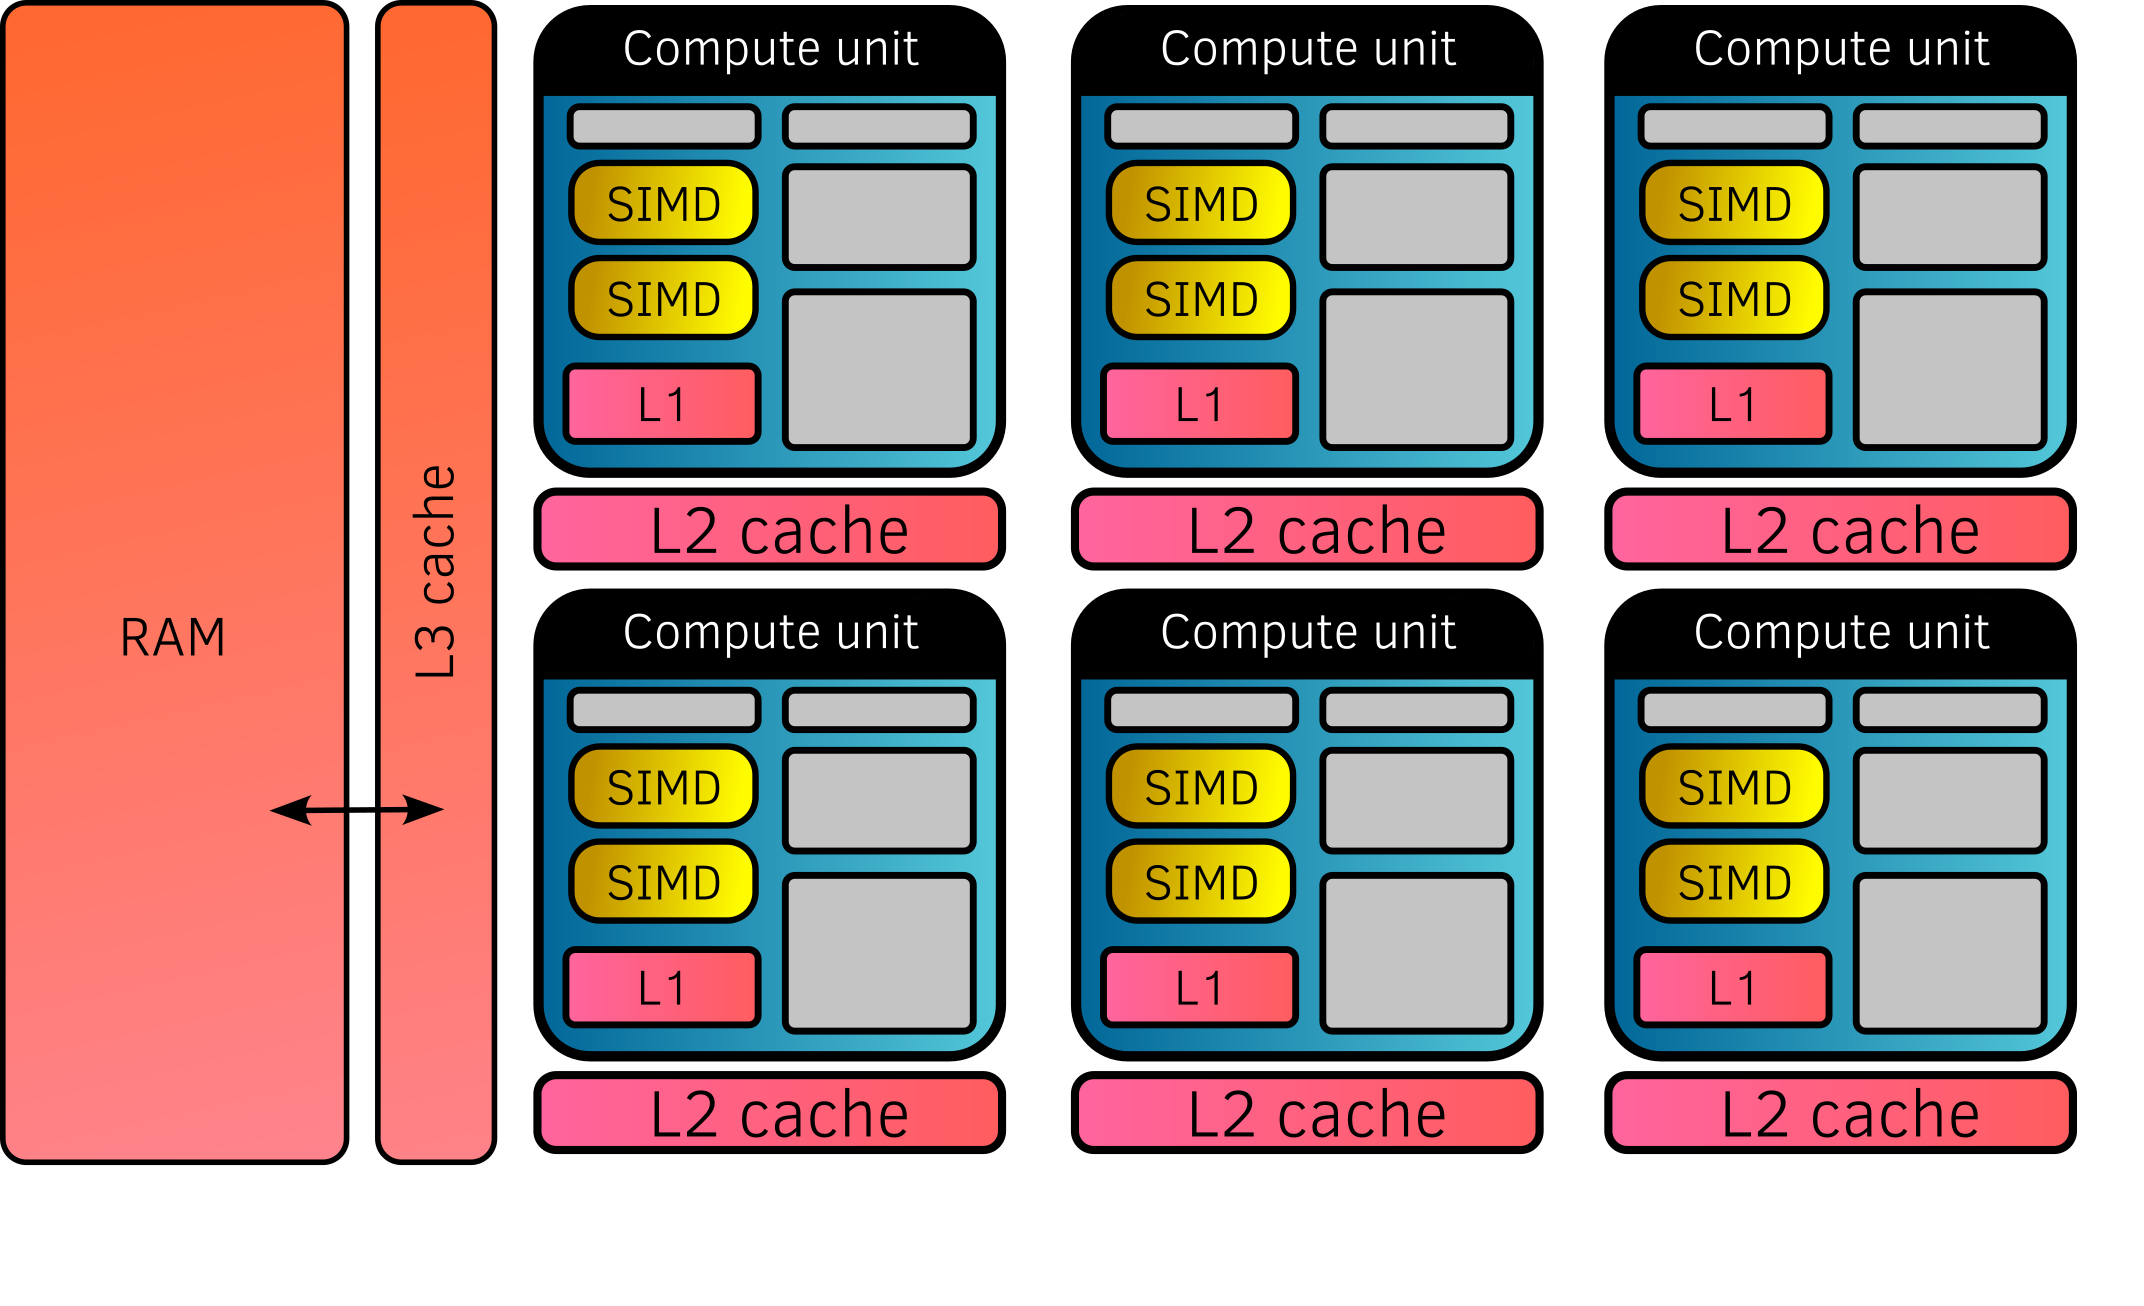
\includegraphics[width=\linewidth]{cpu_architecture.png}
            \end{center}
        \end{column}
        \begin{column}{0.5\linewidth}
            \begin{itemize}
                \item CPUs are for general purpose
                \begin{itemize}
                    \item Sequential task
                    \item Parallel computing
                    \item Operating system
                \end{itemize}
                \item Tens to hundred of cores in biggest processors
                \item SIMD (Single Instruction Multiple Data) units to accelerate arithmetic operations
            \end{itemize}
        \end{column}
    \end{columns}
\end{frame}

% _____________________________________________________________________________

\begin{frame}{Zoom on the GPU architecture}
    \begin{columns}
        \begin{column}{0.5\linewidth}
            \begin{center}
                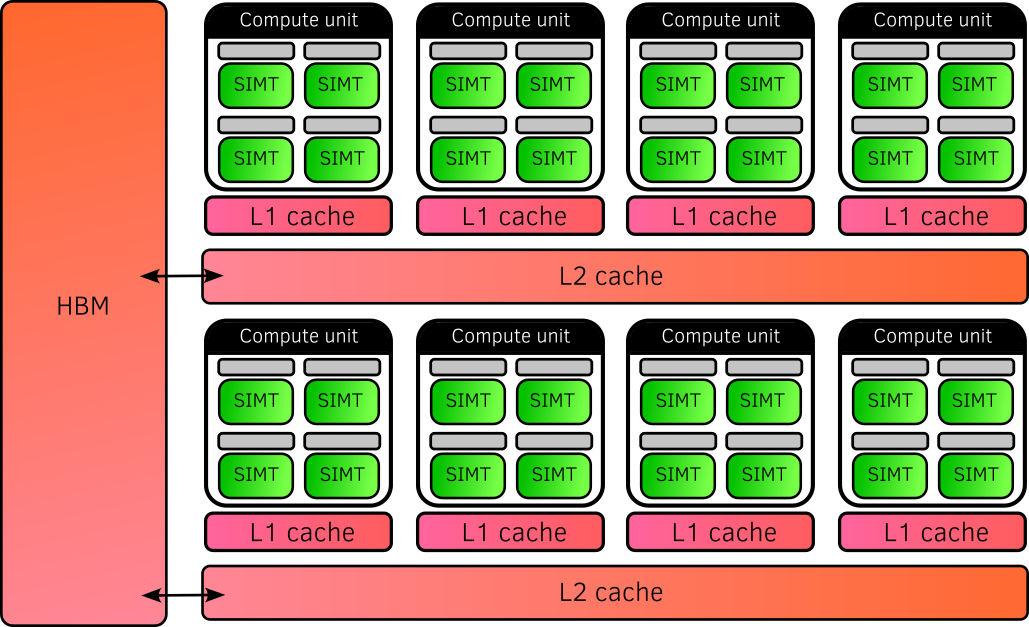
\includegraphics[width=\linewidth]{gpu_architecture.png}
            \end{center}
        \end{column}
        \begin{column}{0.5\linewidth}
            \begin{itemize}
                \item GPUs are designed to achieve massive parallelism of simple kernels
                \item Hundreds of computing units, thousands of threads
                \item Large SIMT vector unit (Single Instruction Multiple Threads) per computing unit
            \end{itemize}
        \end{column}
    \end{columns}
\end{frame}

% _____________________________________________________________________________

\begin{frame}{Main difference between CPU and GPU}
    \begin{center}
        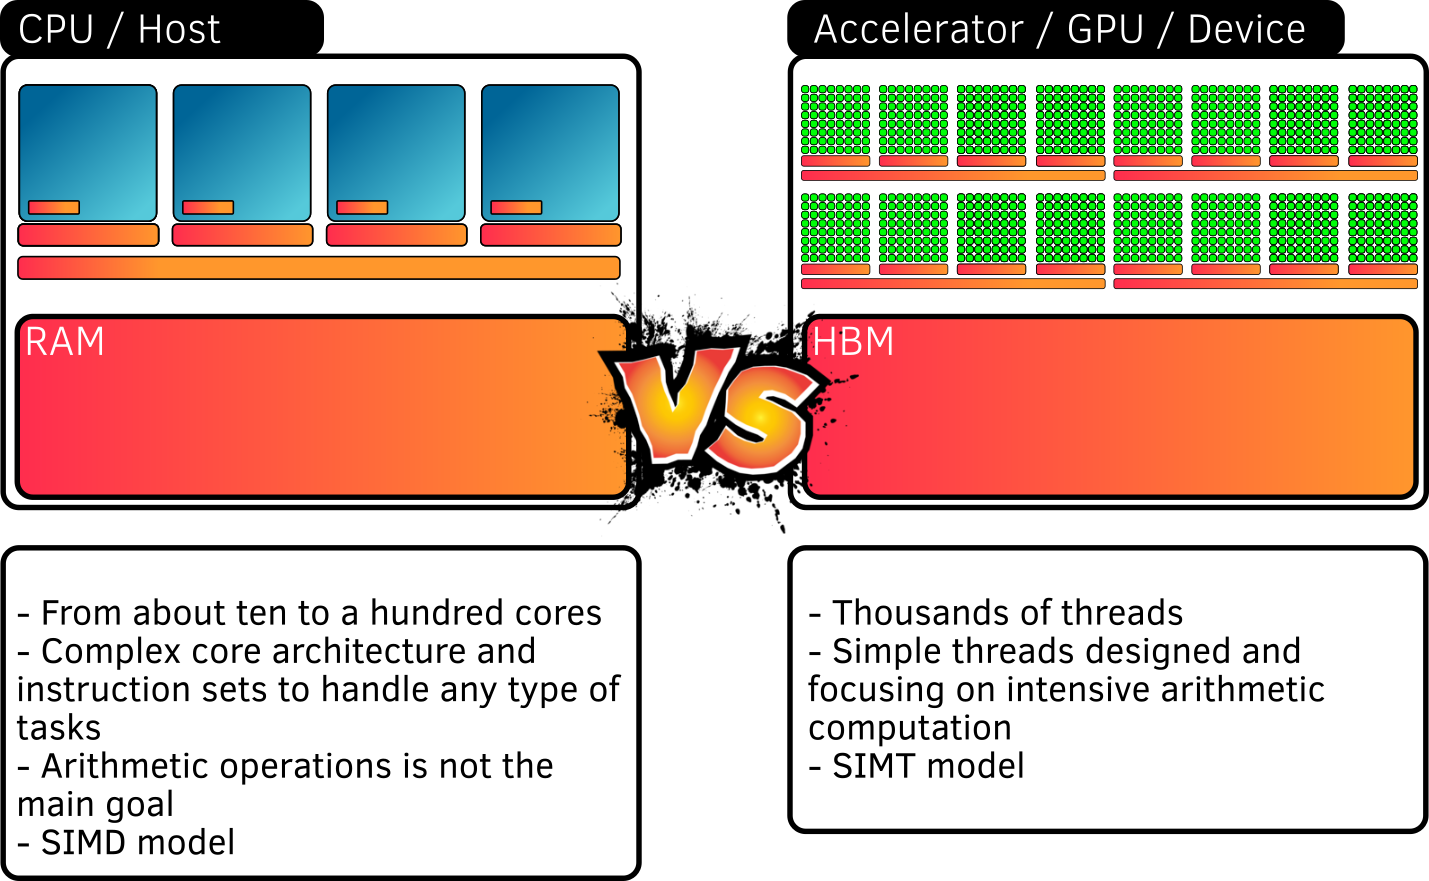
\includegraphics[width=0.8\textwidth]{cpu_vs_gpu.png}
    \end{center}
\end{frame}

% _____________________________________________________________________________

\begin{frame}{Host/device model}
    \begin{itemize}
        \item The program is always started first on the CPU
        \item Today's GPUs \highlight{cannot} work standalone
        \item The CPU is often referred to as the \highlight{Host}
        \item The CPU orchestrates when the kernels are launched on the GPU and how to make the memory transfers
        \item The GPU waits for kernels to execute
        \item The GPU is often referred to as the \highlight{Device}
    \end{itemize}
\end{frame}

% _____________________________________________________________________________

\begin{frame}{SIMD versus SIMT}
    \begin{center}
        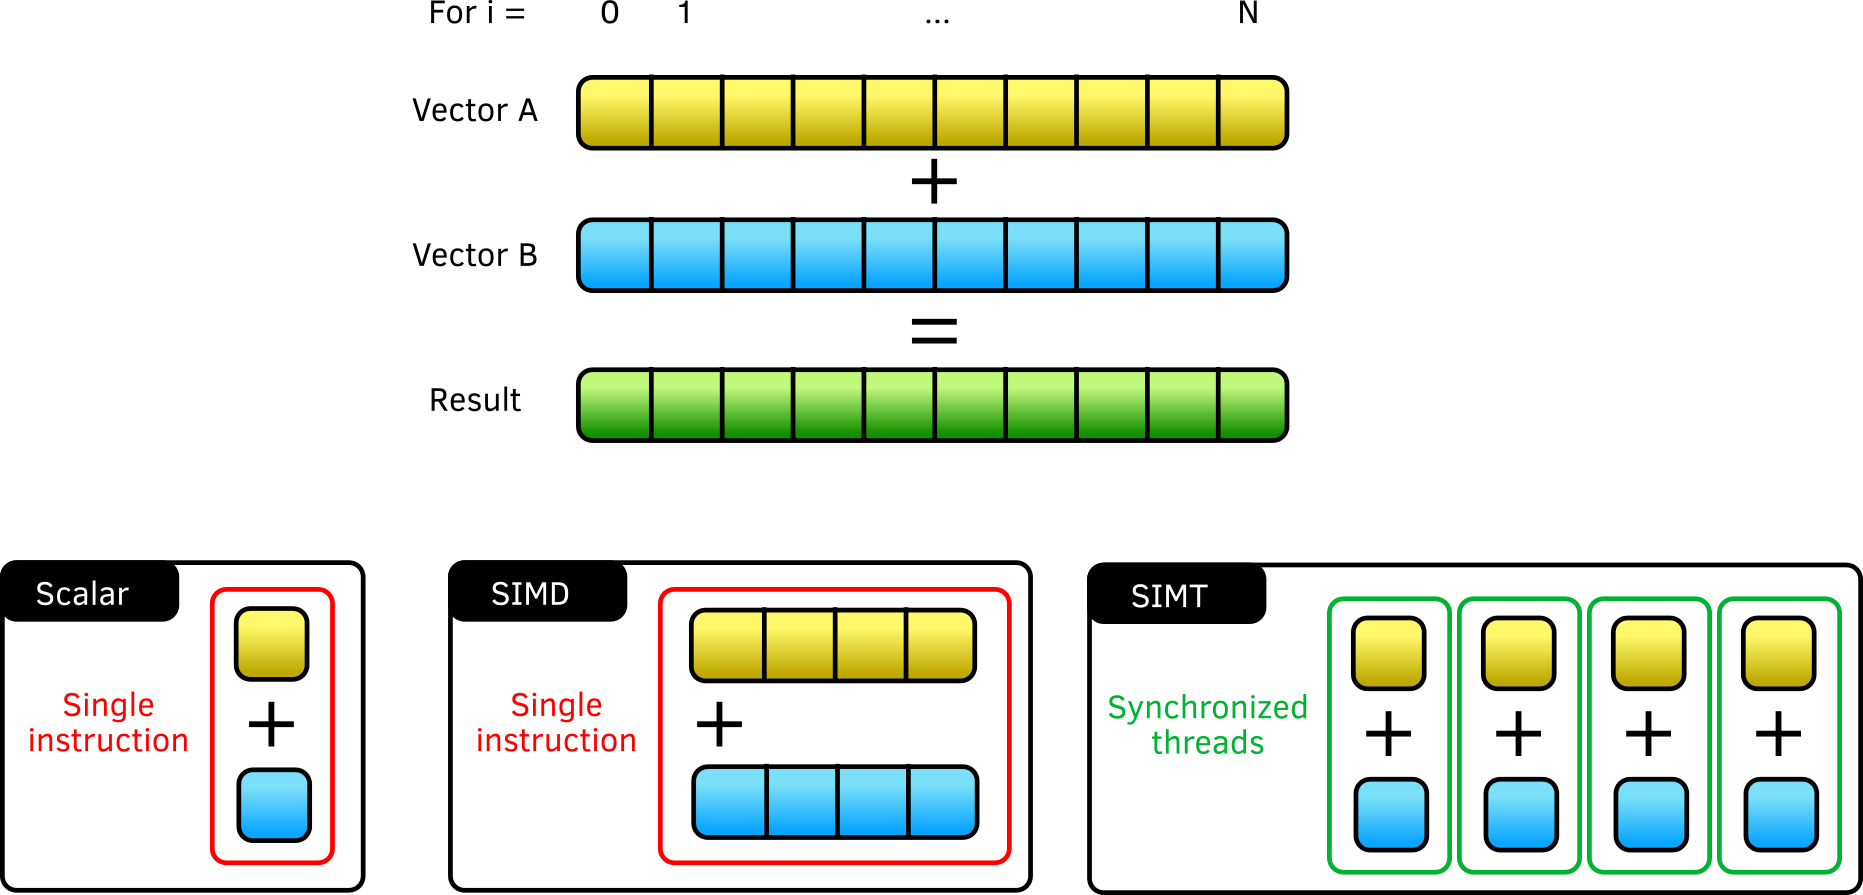
\includegraphics[width=\textwidth]{SIMD_vs_SIMT.png}
    \end{center}
\end{frame}

% _____________________________________________________________________________

\begin{frame}{What's the motivation of putting GPUs in supercomputers?}
    \begin{center}
        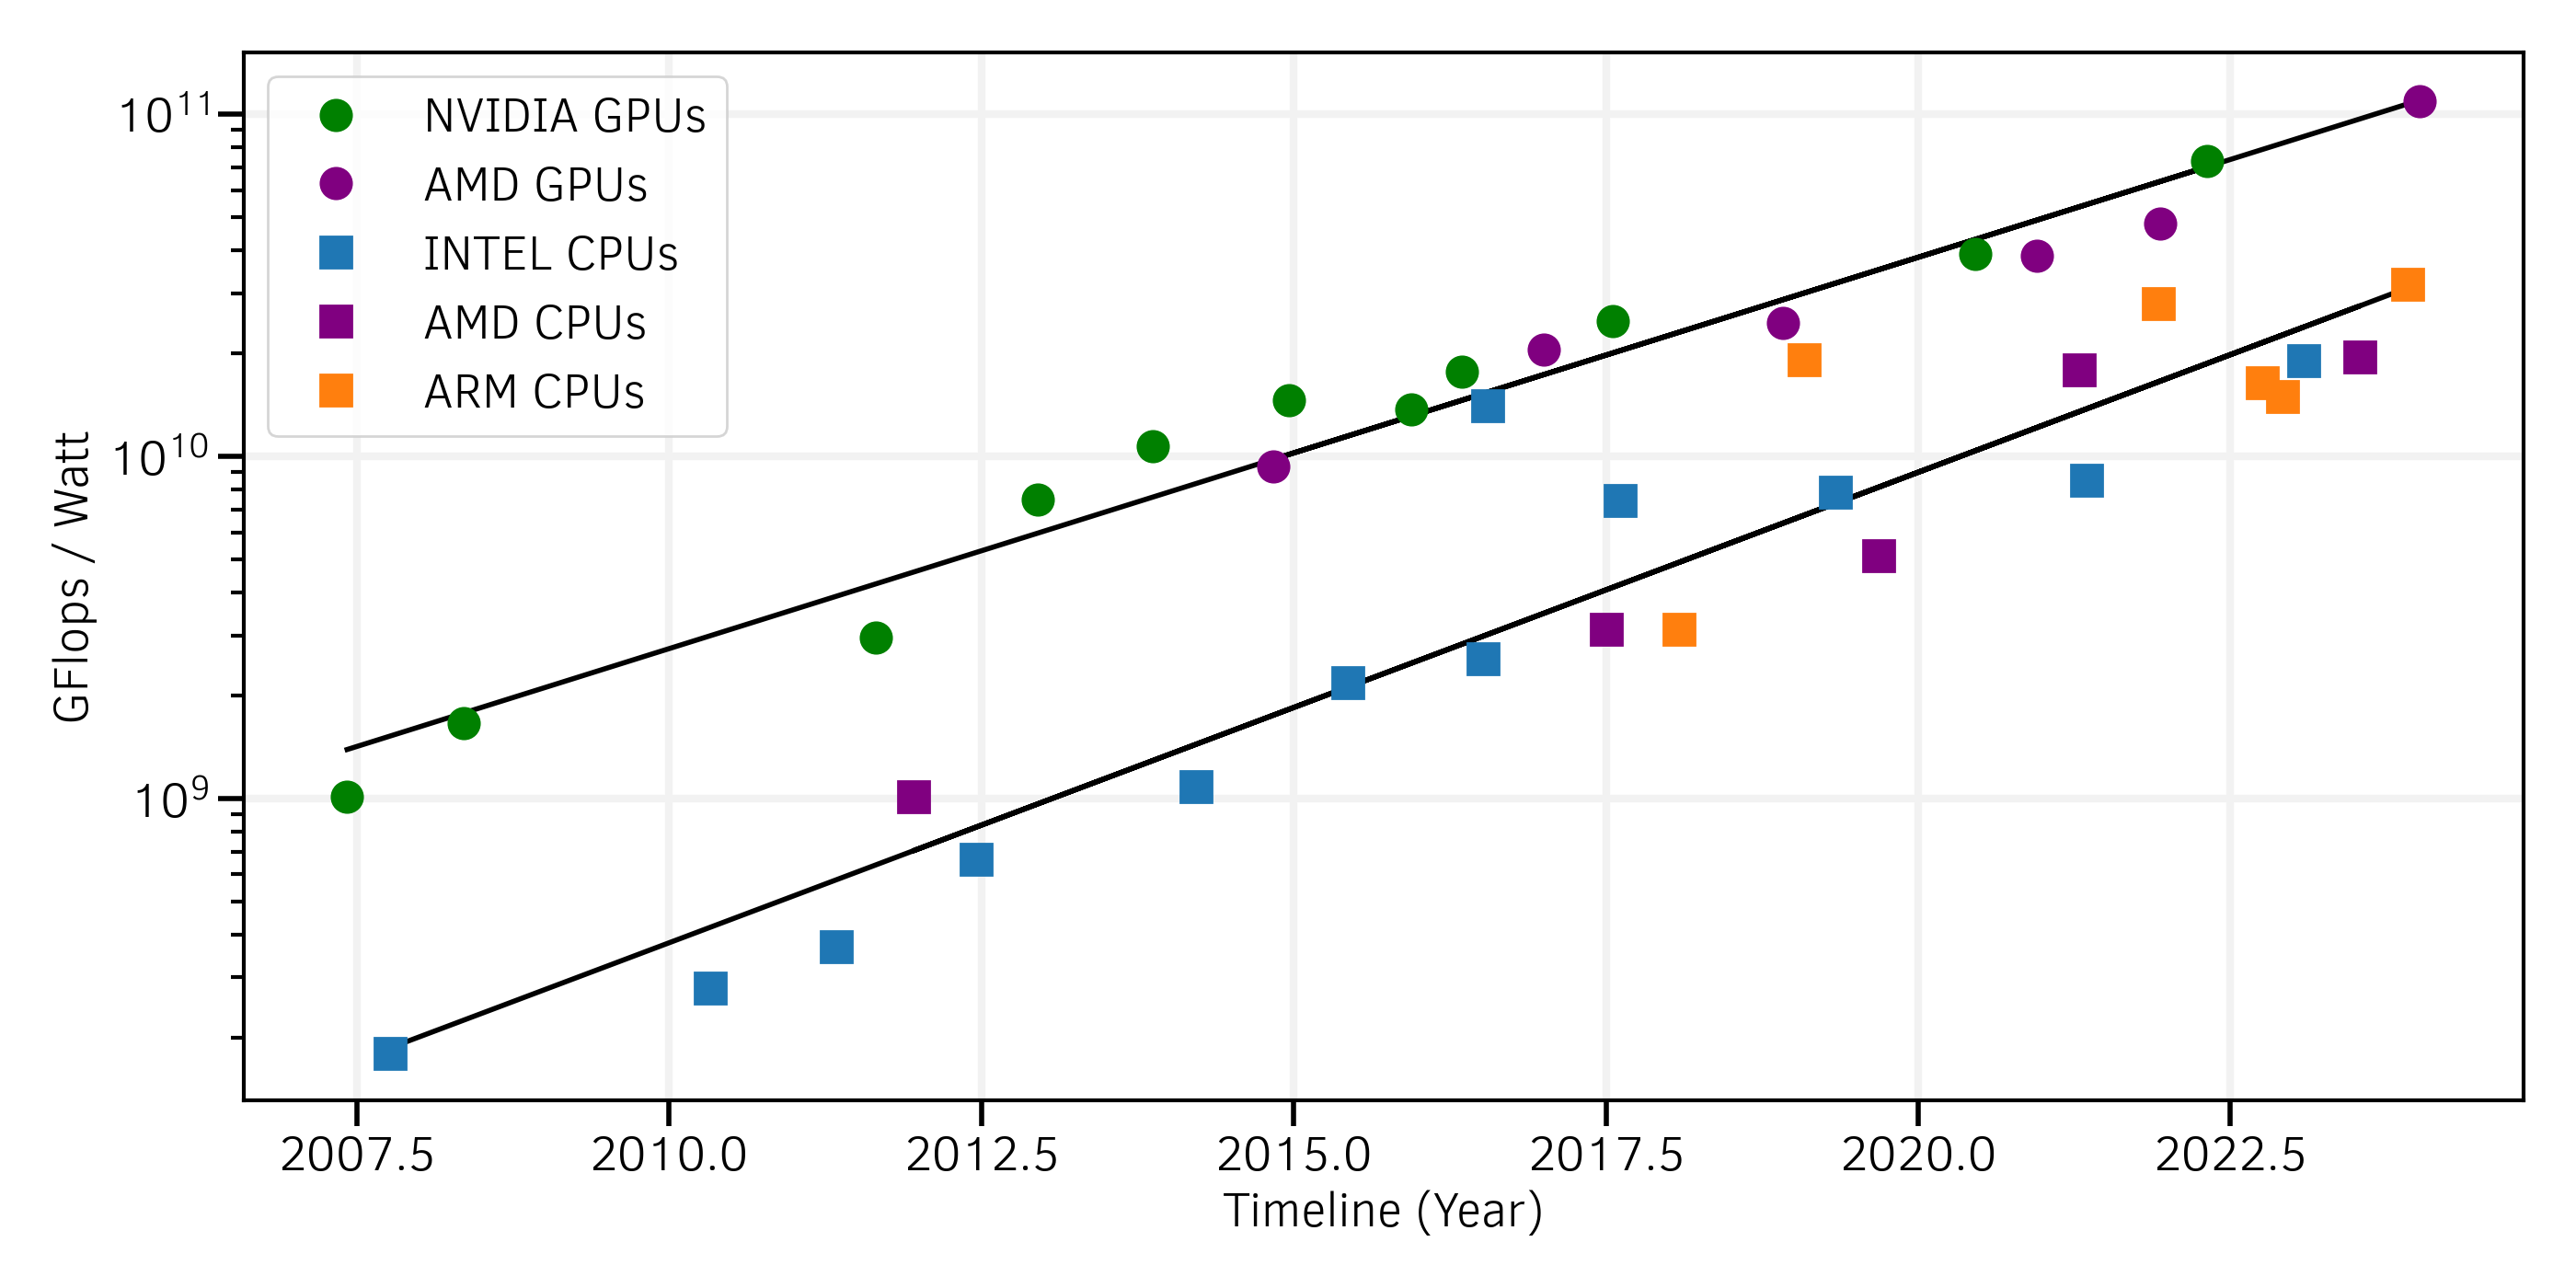
\includegraphics[width=0.8\textwidth]{flop_watt_ratio_history_fp64.png}
    \end{center}

    \structure{Question:} How to build the fastest machine with the lowest power consumption and the lowest cost?
\end{frame}

% _____________________________________________________________________________

\begin{frame}{Parallel programming models and libraries in numerical science}
    \begin{center}
        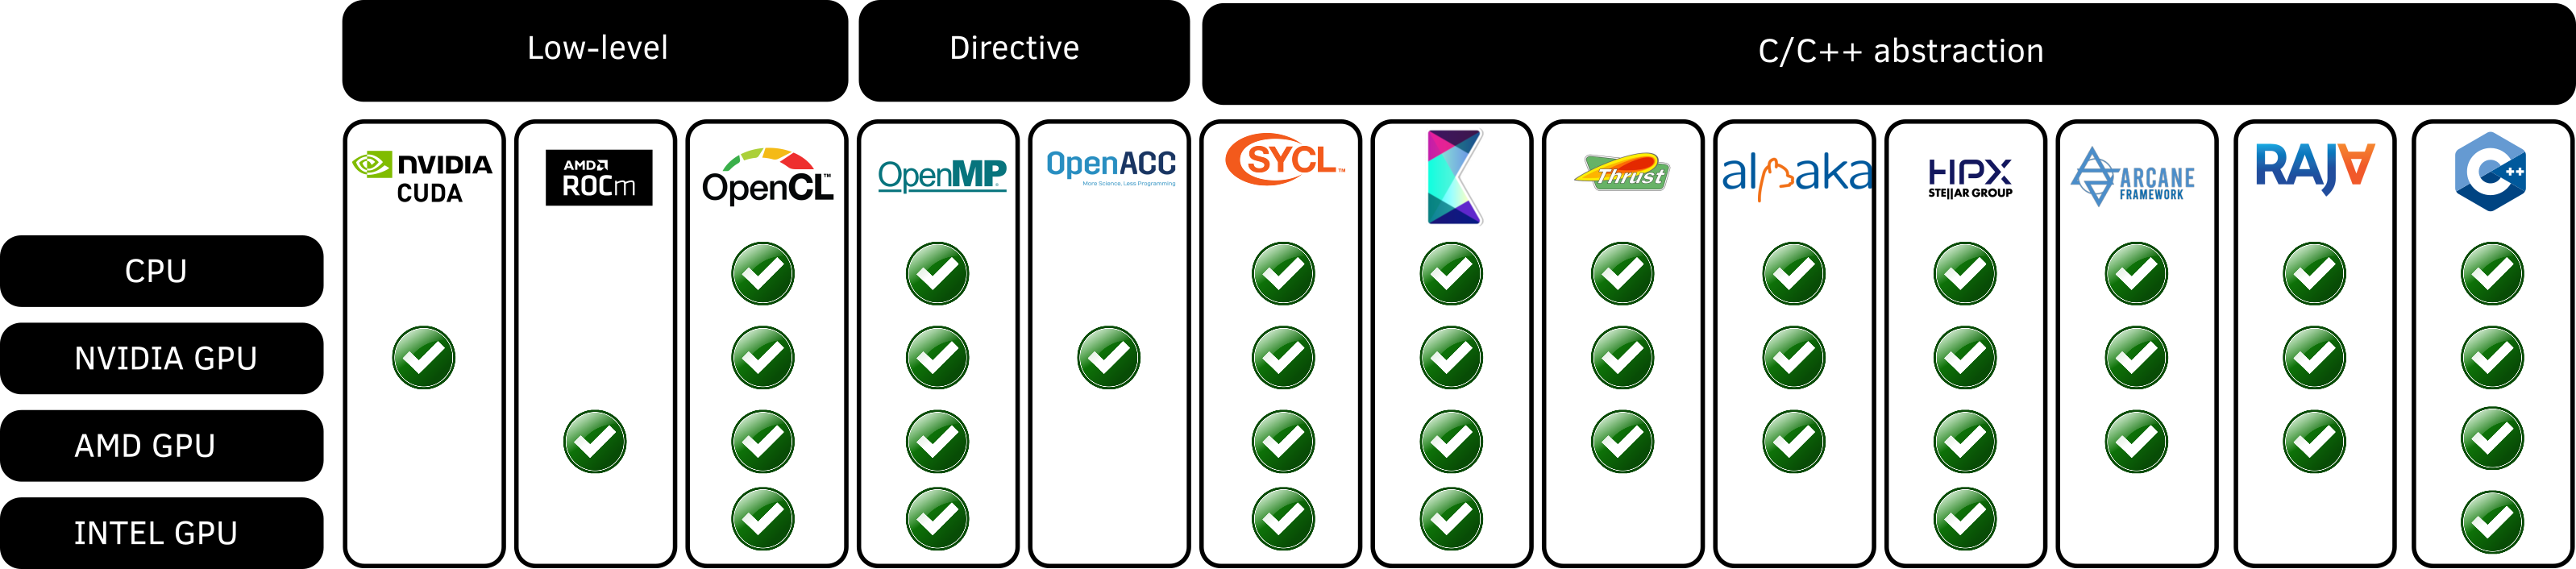
\includegraphics[width=\textwidth]{prog_model.png}
    \end{center}
    \begin{itemize}
        \item Performance portability is one thing
        \item But we will see that developers need more
    \end{itemize}
\end{frame}

% _____________________________________________________________________________

\begin{frame}{Performance, portability and productivity}
    \begin{columns}[T]
        \begin{column}{0.45\linewidth}
            What \emph{every developer} want

            \vspace{1em}

            \begin{description}[Performance]
                \item[Performance] Get the best performance on a specific hardware
                \item[Portability] Run the same code on different hardware
                \item[Productivity] Write code quickly and easily, maintain and extend code, leverage architecture optimization
            \end{description}
        \end{column}
        \begin{column}{0.55\linewidth}
            What \emph{developers for science} also want

            \vspace{1em}

            \begin{description}[Interporability]
                \item[Maturity] Production-ready (i.e. not research product)
                \item[Community] Contributors, support, documentation, examples
                \item[Longevity] Long-term maintenance, bug fixes, updates, sponsorship
                \item[Interporability] Possibility to easily couple with other libraries and tools (IO, Linear Algebra, Machine Learning, etc.)
            \end{description}
        \end{column}
    \end{columns}
\end{frame}

% _____________________________________________________________________________

\begin{frame}{Do \emph{you} need performance portability?}
    \begin{columns}[T]
        \begin{column}{0.5\linewidth}
            Probably \emph{yes} if you...

            \vspace{1em}

            \begin{itemize}
                \item Want your code to run on different hardware technologies (CPU, GPU)
                \item Have performance requirements
                \item Cannot afford to maintain and optimize different versions of your code for each possible hardware of the market
                \item Want to focus on algorithmic and not on code development
                \item Want your code to be easily maintainable and readable by others, especially non experts
            \end{itemize}
        \end{column}
        \begin{column}{0.5\linewidth}
            Maybe \emph{no} if you...

            \vspace{1em}

            \begin{itemize}
                \item Need to tune your algorithms to work as fast as possible on a given hardware
                \item Want to explore a new architecture
            \end{itemize}
        \end{column}
    \end{columns}
\end{frame}

% _____________________________________________________________________________

\begin{frame}{Kokkos programming model}
    Kokkos is a performance portability parallel programming model build upon the C++-17 standard, designed to abstract already existing parallel programming models

    \vspace{0.5em}

    \begin{center}
        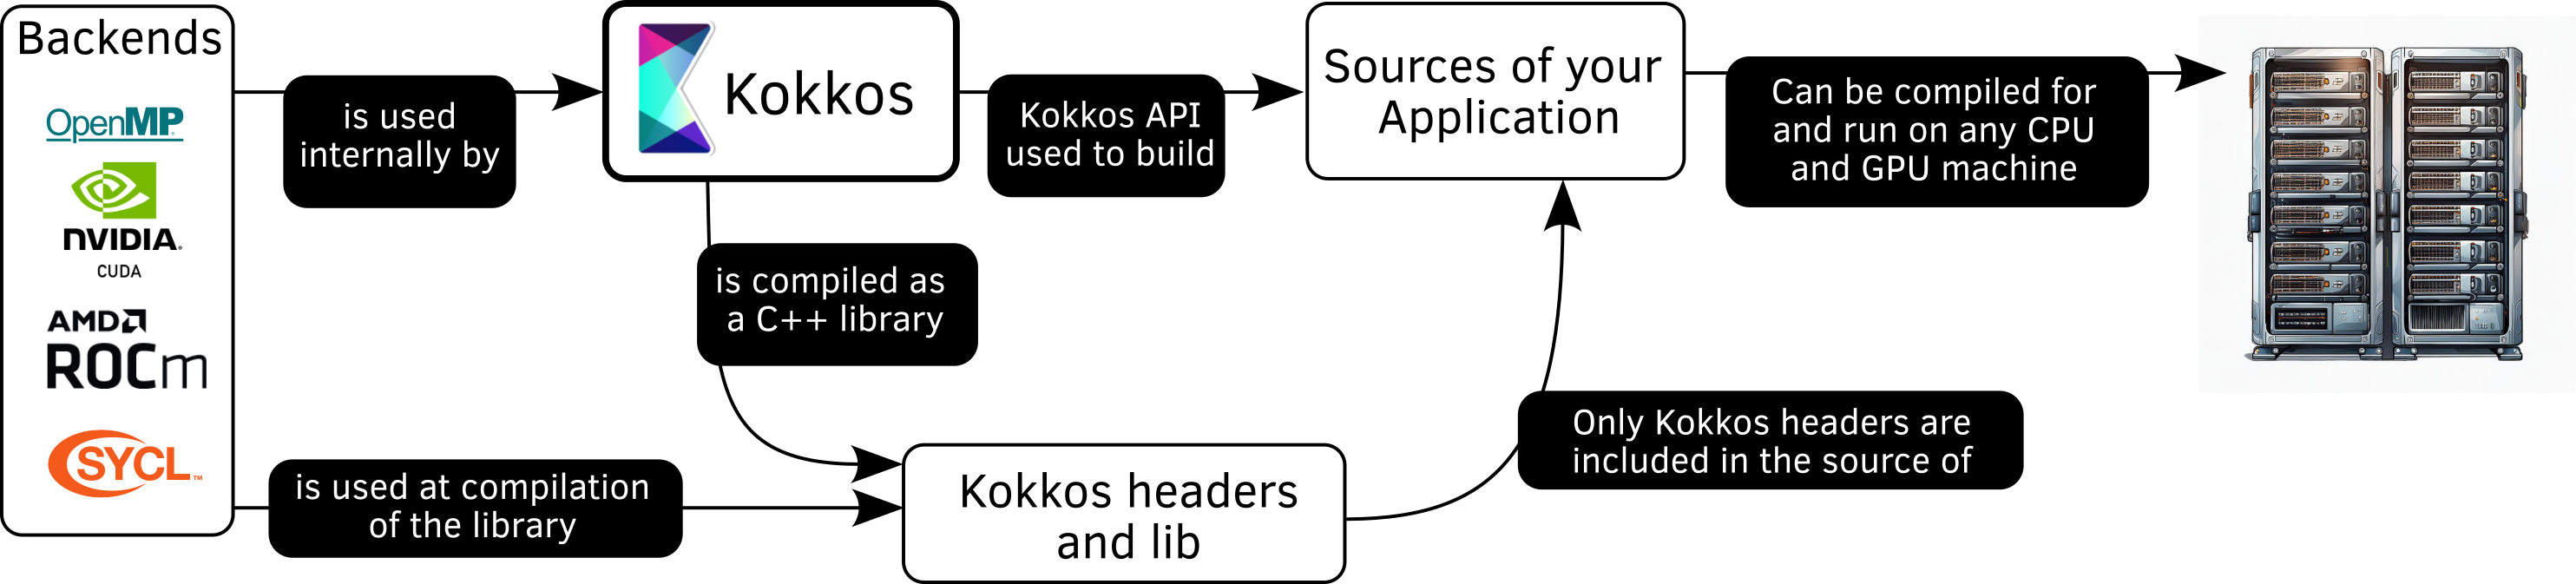
\includegraphics[width=0.9\textwidth]{kokkos_model.png}
    \end{center}
    \begin{itemize}
        \item Kokkos provides data structures and functions based on modern C++ to build your application
        \item Developers never directly use underlying backends (no CUDA kernels for instance)
    \end{itemize}
\end{frame}

% _____________________________________________________________________________

\begin{frame}{Kokkos parallelism scope}
    \begin{itemize}
        \item Kokkos only handle node-level parallelism
        \item You still need a model for distributed memory parallelism (e.g. MPI)
    \end{itemize}
\end{frame}

% _____________________________________________________________________________

\begin{frame}{Kokkos: a tool for both C++ beginners and experts}
    \begin{itemize}
        \item Kokkos' basic capabilities
        \begin{itemize}
            \item Abstraction of most parallel patterns used in HPC (loops, reduction, scan)
            \item Abstracted basic data structures used in science (vectors, multidimensional arrays, sub-arrays, strided arrays, etc)
        \end{itemize}
        \item Kokkos' advanced capabilities
        \begin{itemize}
            \item Advanced data structure properties
            \item Thread safety, thread scalability, and atomic operations
            \item Hierarchical patterns for maximizing parallelism
        \end{itemize}
        \item Kokkos' tools and Kernels
        \begin{itemize}
            \item Profiling, tuning and debuging tools
            \item Interacting with Python and Fortran
            \item Library extensions: Kokkos-Kernels for Linear Algebra, Kokkos-FFT, Kokkos-Comm and more
        \end{itemize}
    \end{itemize}
\end{frame}

% _____________________________________________________________________________

\begin{frame}{Kokkos ecosystem}
    \begin{center}
        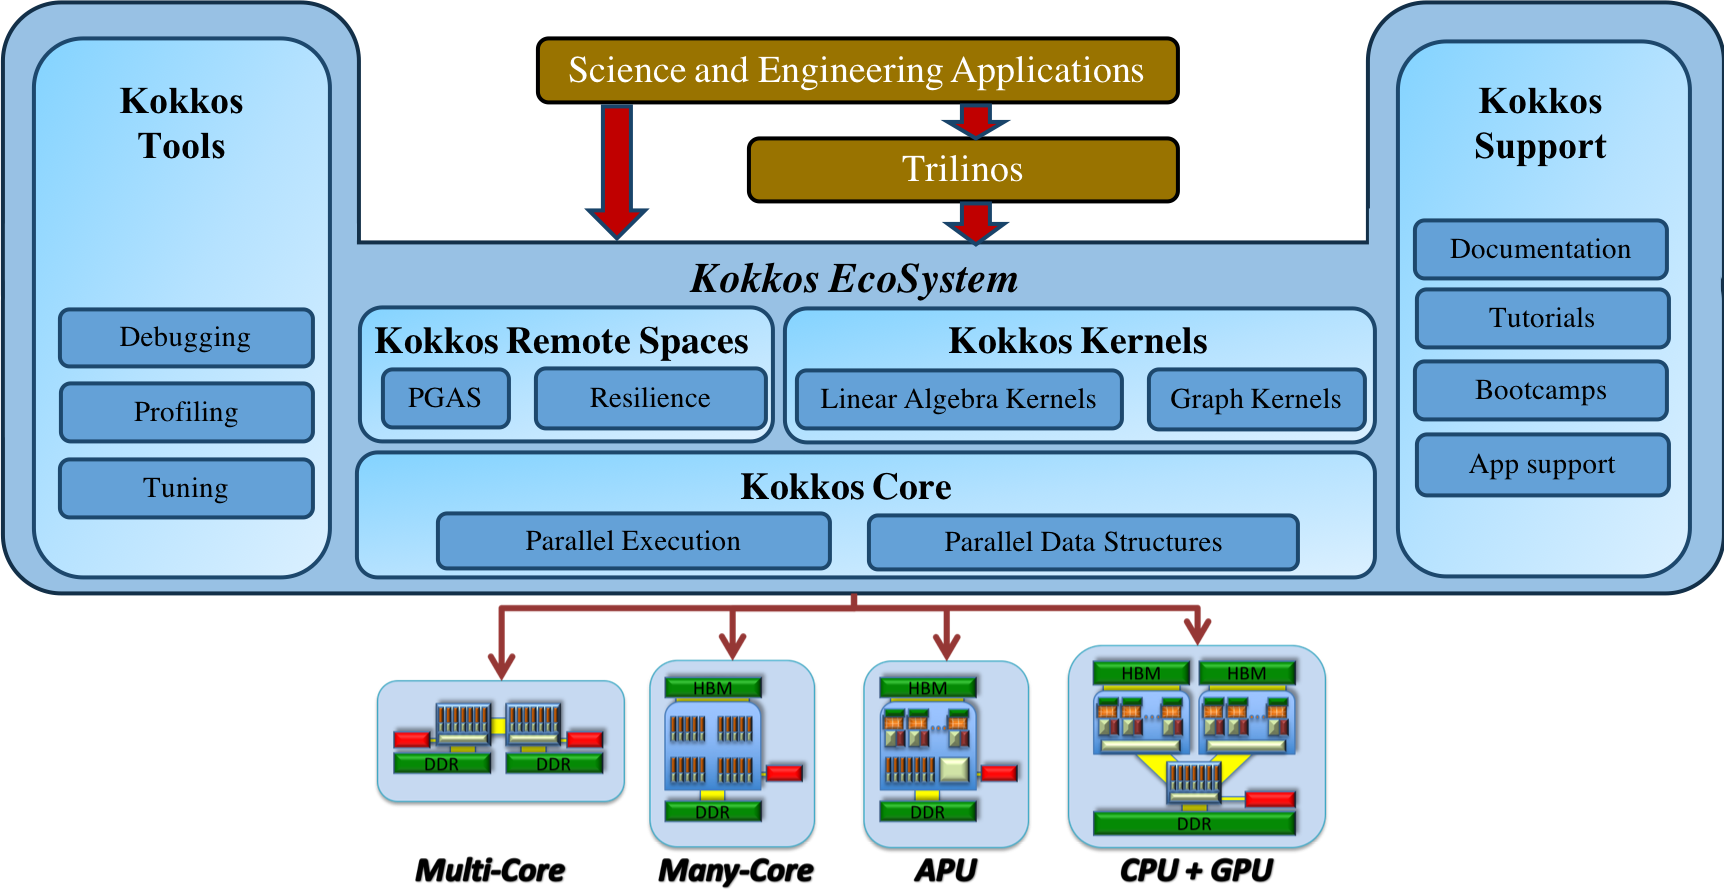
\includegraphics[width=0.9\textwidth]{kokkos-ecosystem.png}
    \end{center}
\end{frame}

% _____________________________________________________________________________

\begin{frame}{Kokkos useful resources}
    \begin{description}[GitHub repository]
        \item[GitHub repository] \githublink{\url{https://github.com/kokkos}}
        \item[Documentation] \doclink{\url{https://kokkos.org/kokkos-core-wiki}}
        \item[Slack channel] \awesomelink{slack}{\url{https://kokkosteam.slack.com}}
        \item[Cheat sheet] \awesomelink{file}{\url{https://cexa-project.org/documents}}
    \end{description}
\end{frame}

% _____________________________________________________________________________

\section{Basic concepts of Kokkos}

% _____________________________________________________________________________

\subsection{Compilation}

% _____________________________________________________________________________

\begin{frame}{Kokkos}
    \begin{itemize}
        \item Source code in the \githublink{\href{https://github.com/kokkos/kokkos}{Kokkos GitHub repository}}
        \item C++ library, mostly header-only
        \item Requires CMake and a C++ compiler
        \item Different ways to add it to your project
        \begin{itemize}
            \item External library
            \item Inline build
            \item Spack
        \end{itemize}
    \end{itemize}
    \begin{center}
        
\includegraphics[height=3em]{GitHub-logo.png}%
        \hspace{1em}%
        
\includegraphics[height=2em]{spack.png}%
    \end{center}
\end{frame}

% _____________________________________________________________________________

\begin{frame}{The notion of backend in Kokkos}
    \begin{itemize}
        \item Kokkos is compiled to target a specific backend
        \item Kokkos is portable until you compile it
        \item You need one compilation per backend
    \end{itemize}
    \begin{center}
        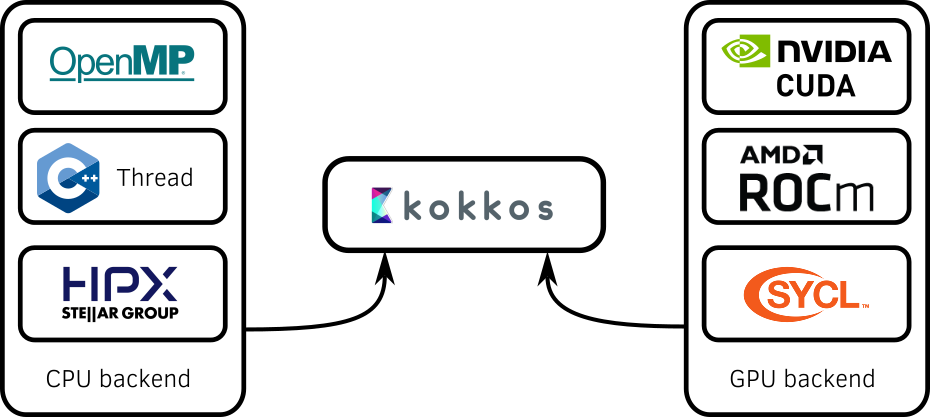
\includegraphics[width=0.6\textwidth]{kokkos_backend.png}
    \end{center}
\end{frame}

% _____________________________________________________________________________

\begin{frame}[fragile]{Compiling Kokkos with the default parameters}
    \begin{columns}
        \begin{column}{0.6\linewidth}
            \begin{itemize}
                \item Defaults to the serial backend
                \item Use the default compiler or specify it with \texttt{-DCMAKE\_CXX\_COMPILER=<command>}
                \item Minimum supported version of the compilers detailed \doclink{\href{https://kokkos.org/kokkos-core-wiki/requirements.html}{in the doc}}
            \end{itemize}
            \begin{minted}{bash}
                cmake \
                    -B ${build_dir} \
                    -DCMAKE_CXX_COMPILER=g++
            \end{minted}
        \end{column}
        \begin{column}{0.4\linewidth}
            \begin{center}
                \begin{tblr}[theme=kokkostable]{ll}
                    Compiler name & Command \\
                    Clang & \texttt{clang++} \\
                    GCC & \texttt{g++} \\
                    Intel LLVM & \texttt{icpx} \\
                    NVHPC & \texttt{nvc++} \\
                    ROCM & \texttt{hipcc} \\
                \end{tblr}
            \end{center}
        \end{column}
    \end{columns}
\end{frame}

% _____________________________________________________________________________

\begin{frame}[fragile]{Compiling Kokkos for a specific backend}
    \begin{columns}
        \begin{column}{0.45\linewidth}
            \begin{itemize}
                \item Add the option \texttt{-DKokkos\_ENABLE\_<BACKEND>=ON} to enable a specific backend
                \item Only one CPU backend and one GPU backend maximum can be compiled at a time
            \end{itemize}
            \begin{minted}[texcomments]{bash}
                cmake \
                    -B ${build_dir} \
                    -DCMAKE_CXX_COMPILER=g++ \
                    -DKokkos_ENABLE_CUDA=ON
            \end{minted}
        \end{column}
        \begin{column}{0.55\linewidth}
            \begin{center}
                \begin{tblr}[theme=kokkostable]{ll}
                    Backend & Option \\
                    Serial & \texttt{-DKokkos\_ENABLE\_SERIAL=ON} \\
                    OpenMP & \texttt{-DKokkos\_ENABLE\_OPENMP=ON} \\
                    Threads & \texttt{-DKokkos\_ENABLE\_THREADS=ON} \\
                    HPX & \texttt{-DKokkos\_ENABLE\_HPX=ON} \\
                    Cuda & \texttt{-DKokkos\_ENABLE\_CUDA=ON} \\
                    HIP & \texttt{-DKokkos\_ENABLE\_HIP=ON} \\
                    SYCL & \texttt{-DKokkos\_ENABLE\_SYCL=ON} \\
                \end{tblr}
            \end{center}
        \end{column}
    \end{columns}
\end{frame}

% _____________________________________________________________________________

    \begin{frame}{Warning regarding the backends}
    \begin{itemize}
        \item All backends \highlight{do not have the same level of maturity}, some are experimental!
        \item The backend environment (for instance CUDA) must be available on the target machine, \highlight{Kokkos does not install it for you}!
    \end{itemize}
\end{frame}

% _____________________________________________________________________________

\begin{frame}{Compiling Kokkos for a specific architecture}
    \begin{columns}
        \begin{column}{0.4\linewidth}
            \begin{itemize}
                \item Add the architecture option \texttt{-DKokkos\_ARCH\_<NAME>=ON}
                \item CPU architecture is optional, for optimization
                \item GPU architecture is mandatory, deduced if device is present
                \item All CMake options are available \doclink{\href{https://kokkos.org/kokkos-core-wiki/keywords.html}{in the doc}}
            \end{itemize}
        \end{column}
        \begin{column}{0.6\linewidth}
            \begin{center}
                \begin{tblr}[theme=kokkostable]{ll}
                    GPU model & Option \\
                    AMD MI300X & \texttt{-DKokkos\_ARCH\_AMD\_GHX942=ON} \\
                    AMD MI250X & \texttt{-DKokkos\_ARCH\_AMD\_GHX90A=ON} \\
                    Intel GPU Max & \texttt{-DKokkos\_ARCH\_INTEL\_PVC=ON} \\
                    NVIDIA H200 & \texttt{-DKokkos\_ARCH\_HOPPER90=ON} \\
                    NVIDIA A100 & \texttt{-DKokkos\_ARCH\_AMPERE80=ON} \\
                    NVIDIA V100 & \texttt{-DKokkos\_ARCH\_VOLTA70=ON} \\
                \end{tblr}
            \end{center}
        \end{column}
    \end{columns}
\end{frame}

% _____________________________________________________________________________

\begin{frame}[fragile]{Real world case}
    \begin{columns}
        \begin{column}{0.475\linewidth}
            \begin{center}
                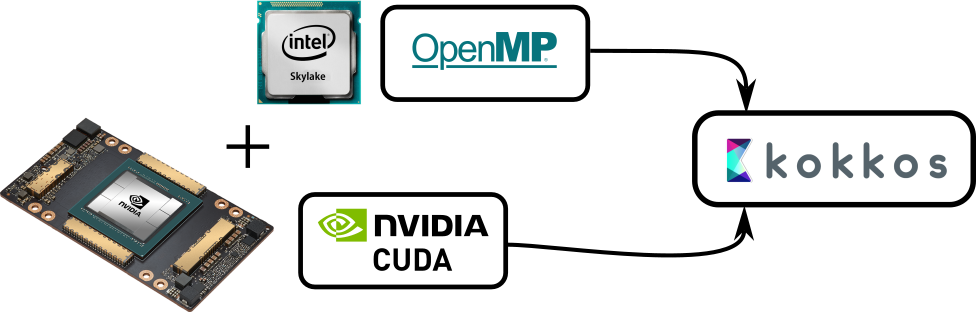
\includegraphics[width=\textwidth]{kokkos_a100_backend.png}
            \end{center}
            \begin{minted}{bash}
                cmake \
                    -B ${build_dir} \
                    -DKokkos_ENABLE_OPENMP=ON \
                    -DKokkos_ARCH_SKX=ON \
                    -DKokkos_ENABLE_CUDA=ON \
                    -DKokkos_ARCH_AMPERE80=ON
            \end{minted}
        \end{column}
        \begin{column}{0.525\linewidth}
            \begin{itemize}
                \item Compiling for a multi-core Xeon Skylake CPU and a A100 NVIDIA GPU
                \item OpenMP option for the multi-core CPU
                \item Skylake option, mostly for vectorization (optional)
                \item CUDA option for the GPU
                \item A100 option, for the correct architecture (mandatory)
            \end{itemize}
        \end{column}
    \end{columns}
\end{frame}

% _____________________________________________________________________________

\begin{frame}{How to add Kokkos to your project}
    \begin{itemize}
        \item There are several ways to do it (for lack of a standard C++ dependency manager)
        \begin{itemize}
            \item Build and install it
            \item As a Git submodule
            \item Using CMake
            \item With Spack
        \end{itemize}
        \item None of them is a perfect solution
    \end{itemize}
\end{frame}

% _____________________________________________________________________________

\begin{frame}{Different ways to treat the Kokkos dependency}
    \begin{columns}[T]
        \begin{column}{0.25\linewidth}
            \strut Build and install it

            \emph{\small\strut(external library)}

            \begin{block}{Pros}
                \begin{itemize}
                    \item You build Kokkos once
                \end{itemize}
            \end{block}
            \begin{alertblock}{Cons}
                \begin{itemize}
                    \item Not flexible
                    \item Not for dev
                    \item Dependency up to the user
                \end{itemize}
            \end{alertblock}
        \end{column}
        \begin{column}{0.25\linewidth}
            \strut As a Git submodule

            \emph{\small\strut(inline build)}

            \begin{block}{Pros}
                \begin{itemize}
                    \item Easy
                    \item Popular
                \end{itemize}
            \end{block}
            \begin{alertblock}{Cons}
                \begin{itemize}
                    \item User may forget to get the submodule
                    \item Not very clean
                \end{itemize}
            \end{alertblock}
        \end{column}
        \begin{column}{0.25\linewidth}
            \strut Using CMake

            \emph{\small\strut(inline build)}

            \begin{block}{Pros}
                \begin{itemize}
                    \item Trivial for the user
                \end{itemize}
            \end{block}
            \begin{alertblock}{Cons}
                \begin{itemize}
                    \item Not trivial for the dev to do it right
                \end{itemize}
            \end{alertblock}
        \end{column}
        \begin{column}{0.25\linewidth}
            \strut With Spack

            \emph{\small\strut(external library)}

            \begin{block}{Pros}
                \begin{itemize}
                    \item Good for production
                    \item Can bring the backend libs
                \end{itemize}
            \end{block}
            \begin{alertblock}{Cons}
                \begin{itemize}
                    \item Not trivial
                    \item Not for dev
                \end{itemize}
            \end{alertblock}
        \end{column}
    \end{columns}
\end{frame}

% _____________________________________________________________________________

\subsection[Starting a Kokkos program]{Starting and compiling a Kokkos program}

% _____________________________________________________________________________

\begin{frame}[fragile]{Start a Kokkos program}
    \begin{columns}
        \begin{column}{0.6\linewidth}
            \begin{minted}{C++}
                #include <Kokkos_Core.hpp>

                int main(int argc, char* argv[]) {
                    Kokkos::initialize(argc, argv);
                    {
                        // Your code here
                    }
                    Kokkos::finalize();
                }
            \end{minted}
        \end{column}
        \begin{column}{0.4\linewidth}
            \begin{itemize}
                \item Include the Kokkos header file (like any other library)
                \item Use the Kokkos namespace \texttt{Kokkos::}
                \item Initialize and finalize Kokkos (like MPI)
            \end{itemize}
        \end{column}
    \end{columns}
\end{frame}

% _____________________________________________________________________________

\begin{frame}[fragile]{Start a Kokkos program (simpler)}
    \begin{columns}
        \begin{column}{0.6\linewidth}
            \begin{minted}{C++}
                #include <Kokkos_Core.hpp>

                int main(int argc, char* argv[]) {
                    Kokkos::ScopeGuard guard(argc, argv);

                    // Your code here
                }
            \end{minted}
        \end{column}
        \begin{column}{0.4\linewidth}
            \begin{itemize}
                \item \texttt{ScopeGuard} is a class that ensures that \texttt{Kokkos::initialize} and \texttt{Kokkos::finalize} are called correctly
                \item Resource Acquisition Is Initialization (RAII) pattern
            \end{itemize}
        \end{column}
    \end{columns}
\end{frame}

% _____________________________________________________________________________

\begin{frame}[fragile]{Use CMake to compile your Kokkos program (simple approach)}
    \begin{columns}
        \begin{column}{0.6\linewidth}
            \begin{minted}{cmake}
                cmake_minimum_required(VERSION 3.21)

                project(my_kokkos_project LANGUAGES CXX)

                find_package(Kokkos REQUIRED)

                add_executable(proj main.cpp)
                target_link_libraries(proj Kokkos::kokkos)
            \end{minted}
        \end{column}
        \begin{column}{0.4\linewidth}
            \begin{itemize}
                \item \texttt{find\_package} command to find Kokkos
                \item \texttt{REQUIRED} aborts the configuration if Kokkos is not found
                \item \texttt{target\_link\_libraries} command to link your program with Kokkos
                \item This is the "Kokkos is built and installed" approach
            \end{itemize}
        \end{column}
    \end{columns}
\end{frame}

% _____________________________________________________________________________

\begin{frame}[fragile]{Making the \texttt{find\_package} part more flexible}
    \begin{columns}
        \begin{column}{0.6\linewidth}
            \begin{minted}[breakafter=/]{cmake}
                find_package(Kokkos CONFIG)
                if(NOT Kokkos_FOUND)
                    include(FetchContent)
                    FetchContent_Declare(
                        kokkos
                        URL https://github.com/kokkos/kokkos/releases/download/4.5.01/kokkos-4.5.01.zip
                    )
                    FetchContent_MakeAvailable(kokkos)
                endif()
            \end{minted}
        \end{column}
        \begin{column}{0.4\linewidth}
            \begin{itemize}
                \item \texttt{find\_package} command to find Kokkos if it's already installed
                \item \texttt{CONFIG} allows to continue if Kokkos is not found
                \item \texttt{FetchContent\_*} commands to download Kokkos if needed
                \item This is the "Kokkos is managed using CMake" approach
            \end{itemize}
        \end{column}
    \end{columns}
\end{frame}

% _____________________________________________________________________________

\begin{frame}[fragile]{Build your Kokkos program}
    \begin{columns}
        \begin{column}{0.6\linewidth}
            \begin{minted}{bash}
                cmake \
                    -B ${build_dir} \
                    -DCMAKE_CXX_COMPILER=${compiler} \
                    <other options>
                cmake \
                    --build ${build_dir} \
                    --parallel ${jobs}
            \end{minted}
        \end{column}
        \begin{column}{0.4\linewidth}
            \begin{itemize}
                \item If Kokkos is installed, it propagates its compilation flags to your program
                \item Otherwise, you specify Kokkos options along with the ones of your program
                \item Build in parallel
            \end{itemize}
        \end{column}
    \end{columns}
\end{frame}

% _____________________________________________________________________________

\begin{exerciseframe}{Exercise 1: First Kokkos program}
    \begin{columns}
        \begin{column}{0.5\linewidth}
            \begin{center}
                
\includegraphics[width=0.9\textwidth]{sleeping_otter.png}
            \end{center}

            Go to the exercise \githublink{\href{https://github.com/CExA-project/cexa-kokkos-tutorials/tree/main/exercises/01_first_program}{01\_first\_program}} and follow the instructions
        \end{column}
        \begin{column}{0.5\linewidth}
            \begin{block}{Goal of this exercise}
                \begin{itemize}
                    \item Write a simple Kokkos program
                    \item Compile the program with CMake for different backends
                    \item Get familiar with the compilation process
                \end{itemize}
            \end{block}
        \end{column}
    \end{columns}
\end{exerciseframe}

\begin{exerciseframe}{Exercise 1: Stepping on Ruche}
    \begin{enumerate}
        \item SSH in the cluster (Windows users without SSH should use KiTTY)
        \begin{minted}{sh}
            ssh login@ruche.mesocentre.universite-paris-saclay.fr
        \end{minted}
        \item Go in the work directory
        \begin{minted}{sh}
            cd $WORKDIR
        \end{minted}
        \item Clone the repo
        \begin{minted}{sh}
            git clone \
                https://github.com/CExA-project/cexa-kokkos-tutorials.git
        \end{minted}
    \end{enumerate}
\end{exerciseframe}

\begin{exerciseframe}{Exercise 1: Ruche environment}
    \begin{itemize}
        \item {\small \doclink{\url{https://github.com/CExA-project/kokkos-training-2025-barcelona}}}
        \item Environment for the hands-on
        \begin{minted}{sh}
            module load gcc/11.2.0/gcc-4.8.5 \
                        cmake/3.28.3/gcc-11.2.0 \
                        cuda/12.2.1/gcc-11.2.0
            export OMP_PROC_BIND=spread \
                   OMP_PLACES=threads
        \end{minted}
        \item Command to run on CPU
        \begin{minted}{sh}
            srun --partition cpu_short --cpus-per-task 20 --pty path/to/exe
        \end{minted}
        \item Command to run on GPU
        \begin{minted}{sh}
            srun --partition gpu --gres gpu:1 --pty path/to/exe
        \end{minted}
    \end{itemize}
\end{exerciseframe}

\begin{exerciseframe}{Exercise 1: Ruche hardware}
    \begin{description}[Documentation]
        \item[Documentation] \doclink{ \url{https://mesocentre.pages.centralesupelec.fr/user_doc/}}
        \item[CPU model] Intel Xeon Gold 6230 (Cascade Lake)
        \item[GPU model] NVIDIA V100
    \end{description}
\end{exerciseframe}

\begin{exerciseframe}{Exercise 1: CMake flags}
    \begin{itemize}
        \item Build with OpenMP
        \begin{minted}{sh}
            cmake -B build_openmp \
                  -DCMAKE_BUILD_TYPE=Release \
                  -DKokkos_ENABLE_OPENMP=ON \
                  -DKokkos_ARCH_NATIVE=ON
            cmake --build build_openmp \
                  --parallel 5
        \end{minted}
        \item Build with Cuda
        \begin{minted}{sh}
            cmake -B build_cuda \
                  -DCMAKE_BUILD_TYPE=Release \
                  -DKokkos_ENABLE_CUDA=ON \
                  -DKokkos_ARCH_VOLTA70=ON
            cmake --build build_cuda \
                  --parallel 5
        \end{minted}
    \end{itemize}
\end{exerciseframe}

% _____________________________________________________________________________

\subsection[Data container]{Data container}

% _____________________________________________________________________________

\begin{frame}[fragile]{Kokkos' abstracted data container}
    \begin{itemize}
        \item Why is it important to have an abstracted data container?
        \begin{itemize}
            \item No need to allocate or deallocate memory by hand
            \item Vendor-specific memory allocation is hidden
            \item Unified semantic and portable memory management (CPU and GPU)
            \item Advanced capabilities (abstracted layout, subarray, multidimensionality, etc.)
        \end{itemize}
        \item Kokkos provides the View class
        \begin{itemize}
            \item View is an abstraction of the notion of container and multidimensional array
            \item Brings portable Python numpy/Fortran-like syntax
        \end{itemize}
    \end{itemize}
\end{frame}

% _____________________________________________________________________________

\begin{frame}[fragile]{Creating a View}
    \begin{columns}
        \begin{column}{0.6\linewidth}
            \begin{minted}{C++}
                Kokkos::View<int[10]>
                    view1("static size");

                Kokkos::View<float*>
                    view2("dynamic size", 10);

                Kokkos::View<double*[10]>
                    view3("static and dynamic size", 10);
            \end{minted}
        \end{column}
        \begin{column}{0.4\linewidth}
            \begin{itemize}
                \item View is a template class
                \item Contains any C++ type (\texttt{int}, \texttt{float}, \texttt{double}, etc)
                \item Number of dimensions fixed at compilation time
                \item Size of each dimension determined at...
                \begin{description}[\texttt{[n]}]
                    \item[\texttt{[n]}] compile time
                    \item[\texttt{*}] runtime
                \end{description}
                \item Name (bonus for debugging!)
            \end{itemize}
        \end{column}
    \end{columns}
\end{frame}

% _____________________________________________________________________________

\begin{frame}[fragile]{Accessing the data}
    \begin{columns}
        \begin{column}{0.6\linewidth}
            \begin{minted}{C++}
                const int Nx = 1000;
                const int Ny = 2000;

                Kokkos::View<int**>
                    my_matrix("matrix", Nx, Ny);

                for (int i = 0; i < Nx; i++) {
                    for (int j = 0; j < Ny; j++) {
                        my_matrix(i, j) = i + j;
                    }
                }
            \end{minted}
        \end{column}
        \begin{column}{0.4\linewidth}
            \begin{itemize}
                \item Data are accessed using the parenthesis operator \texttt{(i, j, k, ...)}
                \item Raw data can be accessed using the \texttt{data()} method (not recommended)
            \end{itemize}
        \end{column}
    \end{columns}
\end{frame}

% _____________________________________________________________________________

\begin{frame}{Where does the data live?}
    \begin{center}
        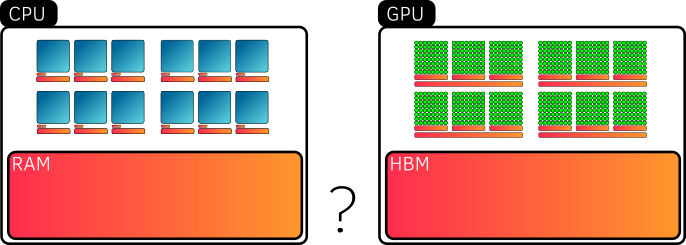
\includegraphics[width=0.65\textwidth]{view_memory.png}
    \end{center}
    \begin{itemize}
        \item A View data lives only in a specific memory space (Host or Device), not both
        \item Suppose we created a view on the Host
    \end{itemize}
\end{frame}

% _____________________________________________________________________________

\begin{frame}{Where does the data live? CPU version}
    \begin{center}
        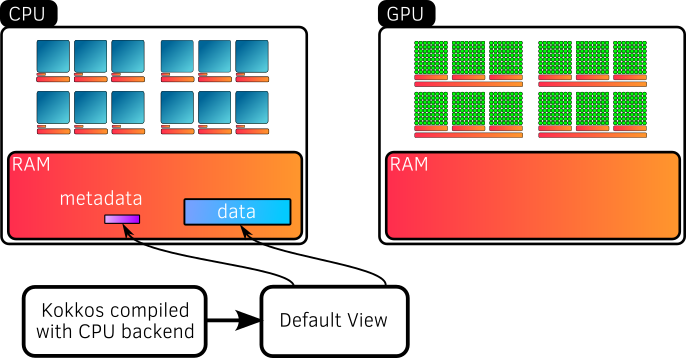
\includegraphics[width=0.65\textwidth]{host_view_memory.png}
    \end{center}
    \begin{itemize}
        \item If Kokkos is compiled with a \highlight{CPU backend only}, the View data is allocated in the \highlight{Host memory} by default
        \item Host view data usually \highlight{cannot} be accessed on the Device
    \end{itemize}
\end{frame}

% _____________________________________________________________________________

\begin{frame}{Where does the data live? GPU version}
    \begin{center}
        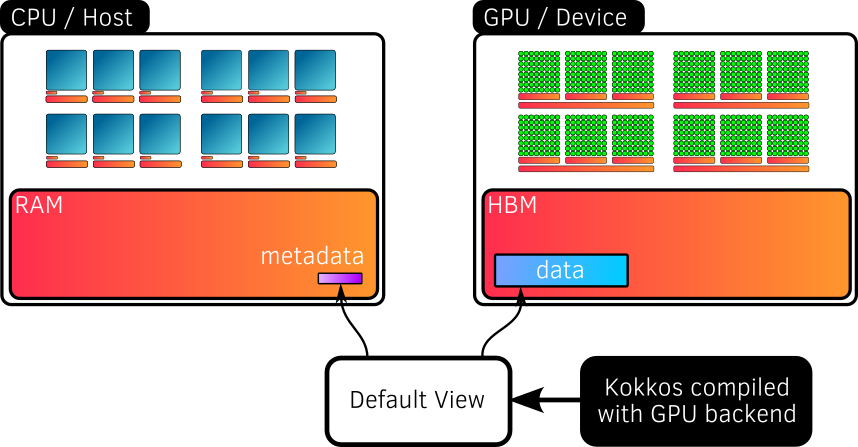
\includegraphics[width=0.65\textwidth]{device_view_memory.png}
    \end{center}
    \begin{itemize}
        \item If Kokkos is compiled with a \highlight{GPU backend}, the View data is allocated in the \highlight{Device memory} by default
        \item Device view data usually \highlight{cannot} be accessed on the Host (we'll see later how to transfer data)
    \end{itemize}
\end{frame}

% _____________________________________________________________________________

\begin{frame}{More about views}
    \begin{itemize}
        \item Allocations only happen when explicitly specified
        \item Copy construction and assignment are shallow: you pass Views by value, not by pointer (e.g. C arrays) or by reference
        \item Reference counting is used for automatic deallocation (like shared pointers)
        \item Views have a \highlight{limited} number of dimensions (up to 7)
    \end{itemize}
\end{frame}

% _____________________________________________________________________________

\begin{frame}[fragile]{Useful methods to manage views}
    \begin{columns}
        \begin{column}{0.45\linewidth}
            \begin{minted}{C++}
                Kokkos::View<int ***>
                    view("view", 10, 20, 30);

                int rank = view.rank();
                assert(rank == 3);

                int size_x = view.extent(0);
                assert(size_x == 10);

                int size = view.size();
                assert(size == 6000);
            \end{minted}
        \end{column}
        \begin{column}{0.55\linewidth}
            \begin{description}[\texttt{extent(dim)}]
                \item[\texttt{rank()}] Return the rank of the view (number of dimensions)
                \item[\texttt{extent(dim)}] Return the number of elements of a specific dimension
                \item[\texttt{size()}] Return the total number of elements
            \end{description}

            \vspace{0.5em}

            And many others not covered in this talk
        \end{column}
    \end{columns}
\end{frame}

% _____________________________________________________________________________

\begin{frame}{Notion of View layout}
    \begin{center}
        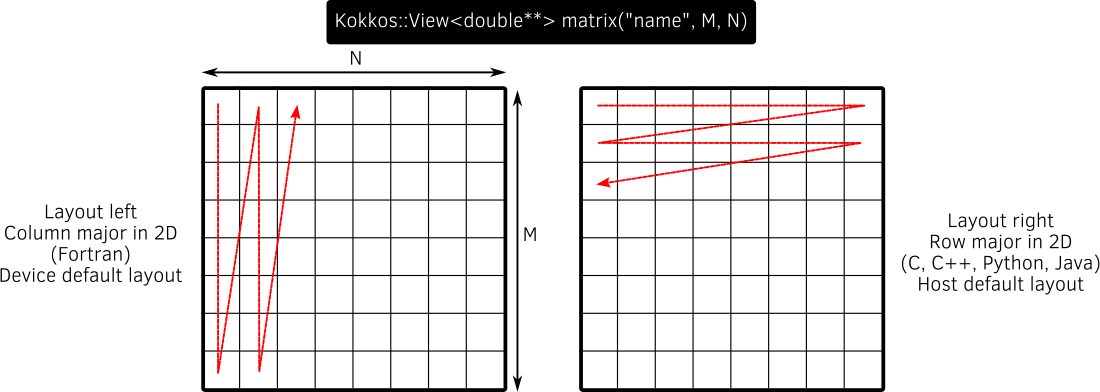
\includegraphics[width=0.8\textwidth]{layout_right_left.png}
    \end{center}
    \begin{itemize}
        \item Layout is the way multidimensional indices map to linear memory
        \item Kokkos provides an abstraction of the data layout
        \item The default layout of a View depends on the backend (Host or Device)
        \item Not covered in this talk
    \end{itemize}
\end{frame}

% _____________________________________________________________________________

\begin{exerciseframe}{Exercise 2: How to use and manage Kokkos Views}
    \begin{columns}
        \begin{column}{0.5\linewidth}
            \begin{center}
                
\includegraphics[width=0.9\textwidth]{sleeping_otter.png}
            \end{center}

            Go to the exercise \githublink{\href{https://github.com/CExA-project/cexa-kokkos-tutorials/tree/main/exercises/02_basic_view}{02\_basic\_view}} and follow the instructions
        \end{column}
        \begin{column}{0.5\linewidth}
            \begin{block}{Goal of this exercise}
                \begin{itemize}
                    \item Create a View
                    \item Manage the view to inspect its metadata
                \end{itemize}
            \end{block}
        \end{column}
    \end{columns}
\end{exerciseframe}

\begin{exerciseframe}{Exercise 2: Ruche environment}
    \begin{itemize}
        \item {\small \doclink{\url{https://github.com/CExA-project/kokkos-training-2025-barcelona}}}
        \item Environment for the hands-on
        \begin{minted}{sh}
            module load gcc/11.2.0/gcc-4.8.5 \
                        cmake/3.28.3/gcc-11.2.0 \
                        cuda/12.2.1/gcc-11.2.0
            export OMP_PROC_BIND=spread \
                   OMP_PLACES=threads
        \end{minted}
        \item Command to run on CPU
        \begin{minted}{sh}
            srun --partition cpu_short --cpus-per-task 20 --pty path/to/exe
        \end{minted}
        \item Command to run on GPU
        \begin{minted}{sh}
            srun --partition gpu --gres gpu:1 --pty path/to/exe
        \end{minted}
    \end{itemize}
\end{exerciseframe}

% _____________________________________________________________________________

\begin{frame}{How to access data living on the Device from the Host?}
    \begin{center}
        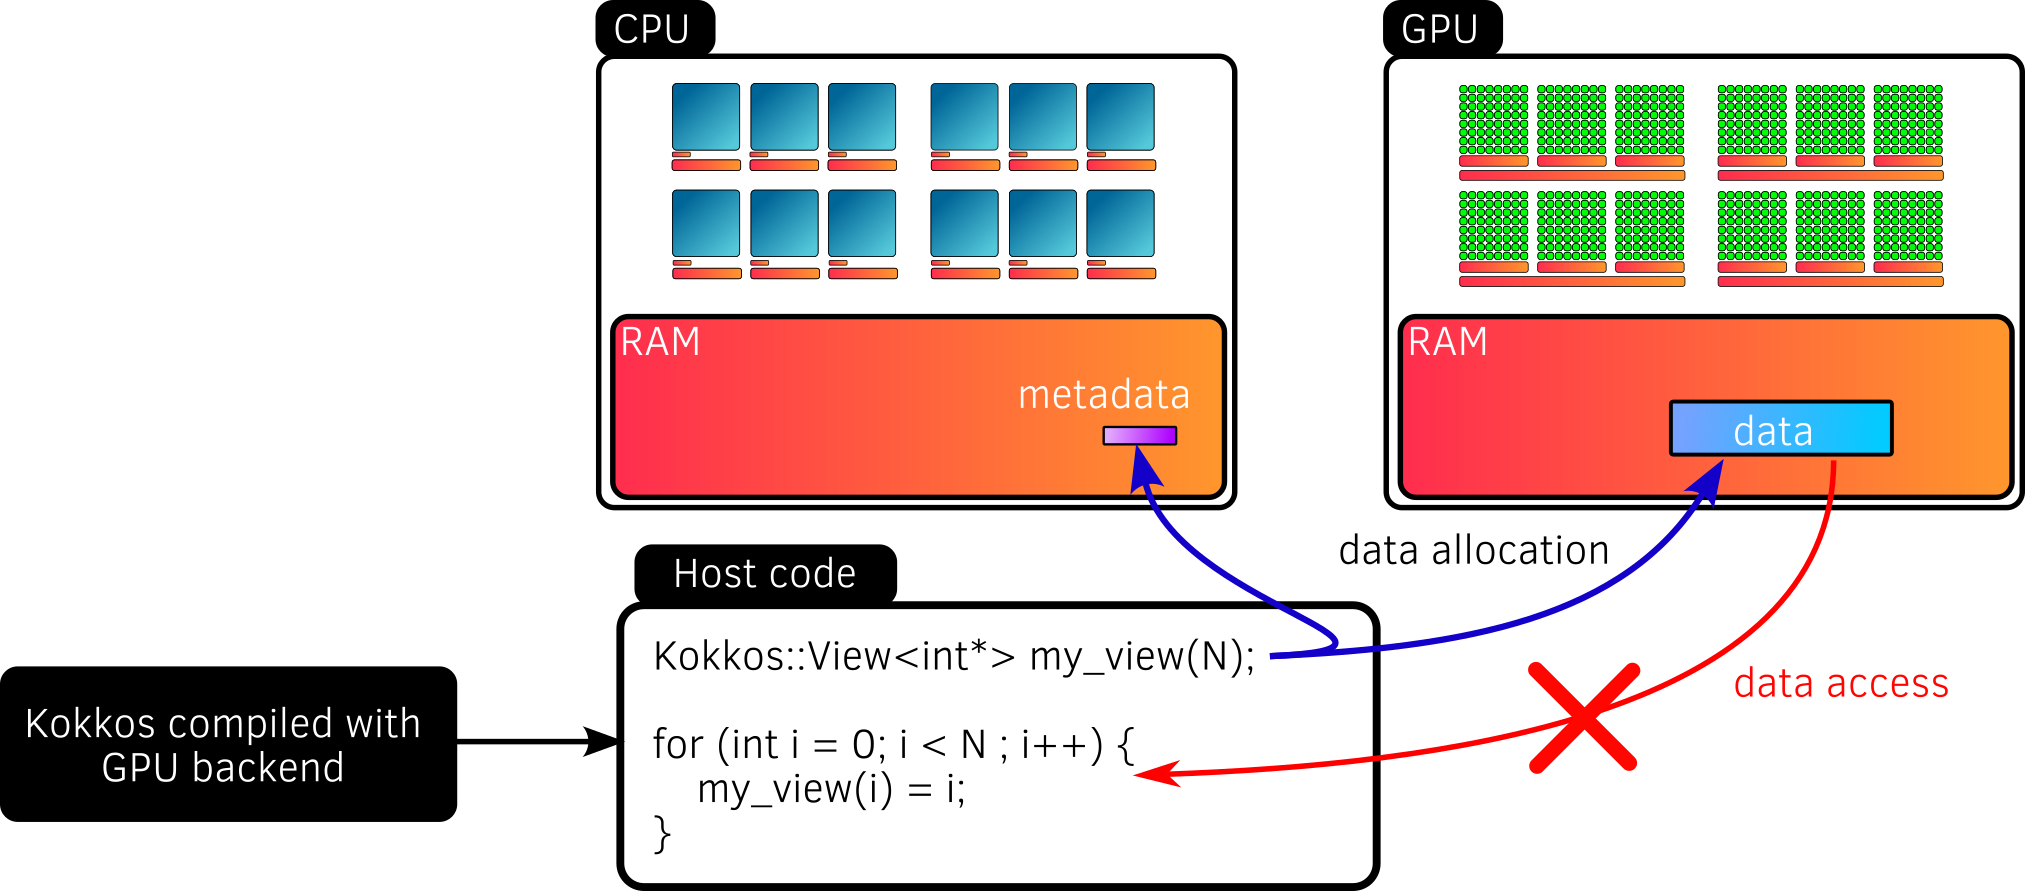
\includegraphics[width=0.9\textwidth]{device_memory_access.png}
    \end{center}

    \structure{Problem:} You cannot!
\end{frame}

% _____________________________________________________________________________

\begin{frame}{The concept of memory space}
    \begin{center}
        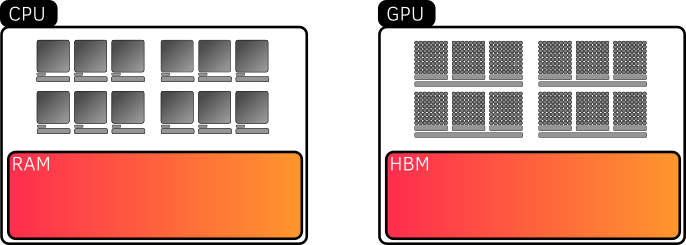
\includegraphics[width=0.7\linewidth]{memory_space.png}
    \end{center}
    \begin{itemize}
        \item Kokkos abstraction for where the data lives: \highlight{memory space}
        \item A View is always associated with a defined memory space (Host or Device) at compile time
        \item By default, view data is allocated
        \begin{itemize}
            \item On the Host if no GPU backend is available
            \item On the Device otherwise
        \end{itemize}
    \end{itemize}
\end{frame}

% _____________________________________________________________________________

\begin{frame}[fragile]{How to set a memory space}
    \begin{columns}
        \begin{column}{0.5\linewidth}
            \begin{minted}{C++}
                Kokkos::View<int**, MemorySpace>
                    my_matrix("matrix", 10, 10);
            \end{minted}
        \end{column}
        \begin{column}{0.5\linewidth}
            \begin{itemize}
                \item Template argument \texttt{MemorySpace} to specify the memory space when creating a view
                \item Several ones available
                \item Using a backend-specific memory space is possible, but it breaks portability
                \item Beginners usually do not need to set it (we'll see why)
            \end{itemize}
        \end{column}
    \end{columns}

    \structure{But:} That's not what you need
\end{frame}

% _____________________________________________________________________________

\begin{frame}[fragile]{All you need is a mirror}
    \begin{columns}
        \begin{column}{0.6\linewidth}
            \begin{minted}{C++}
                Kokkos::View<int**>
                    device_matrix("matrix", 10, 10);

                auto host_matrix =
                    Kokkos::create_mirror(device_matrix);
            \end{minted}

        \end{column}
        \begin{column}{0.4\linewidth}
            \begin{itemize}
                \item A \highlight{mirror view} represents a view in a different memory space
                \item Created with \texttt{create\_mirror}
                \item Similar to its original view (shape, layout, etc.)
                \item Used to create a mirror of a device view on the host
            \end{itemize}
        \end{column}
    \end{columns}
\end{frame}

% _____________________________________________________________________________

\begin{frame}{How to access data living on the Device from the Host?}
    \begin{center}
        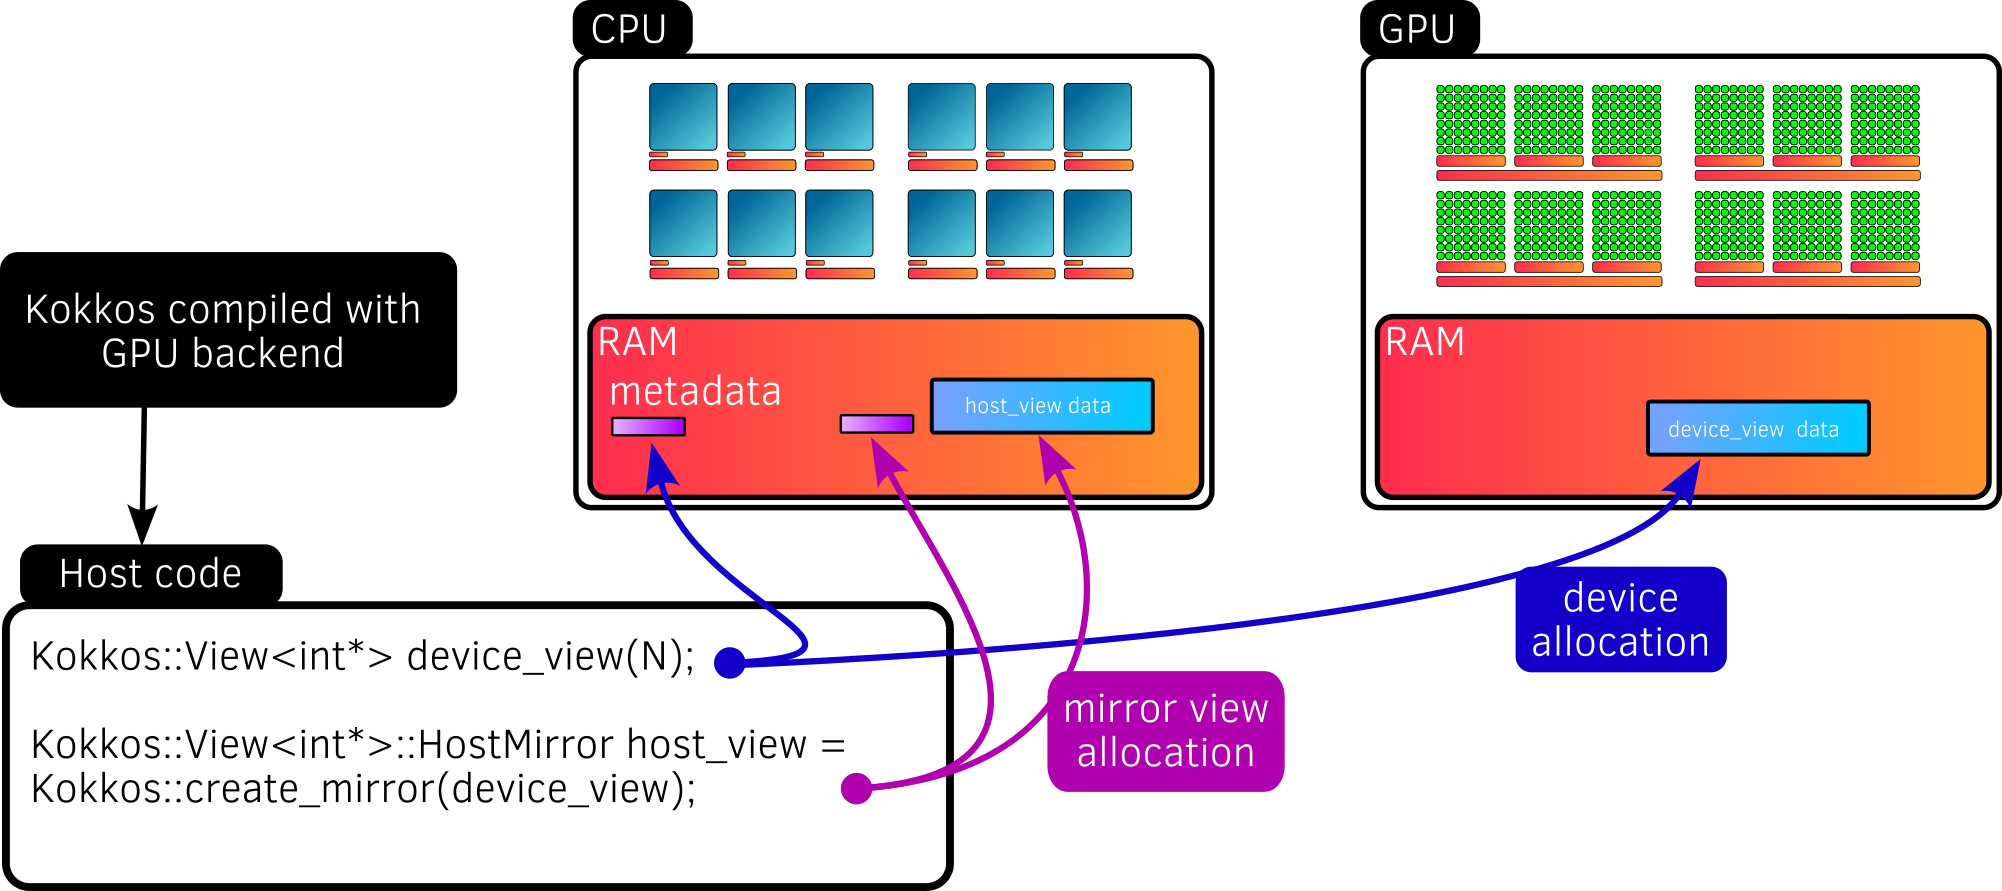
\includegraphics[width=0.9\textwidth]{device_mirror_view.png}
    \end{center}

    \structure{Solution:} With a mirror view!
\end{frame}

% _____________________________________________________________________________

\begin{frame}{How to access data living on the Host from the Host?}
    \begin{center}
        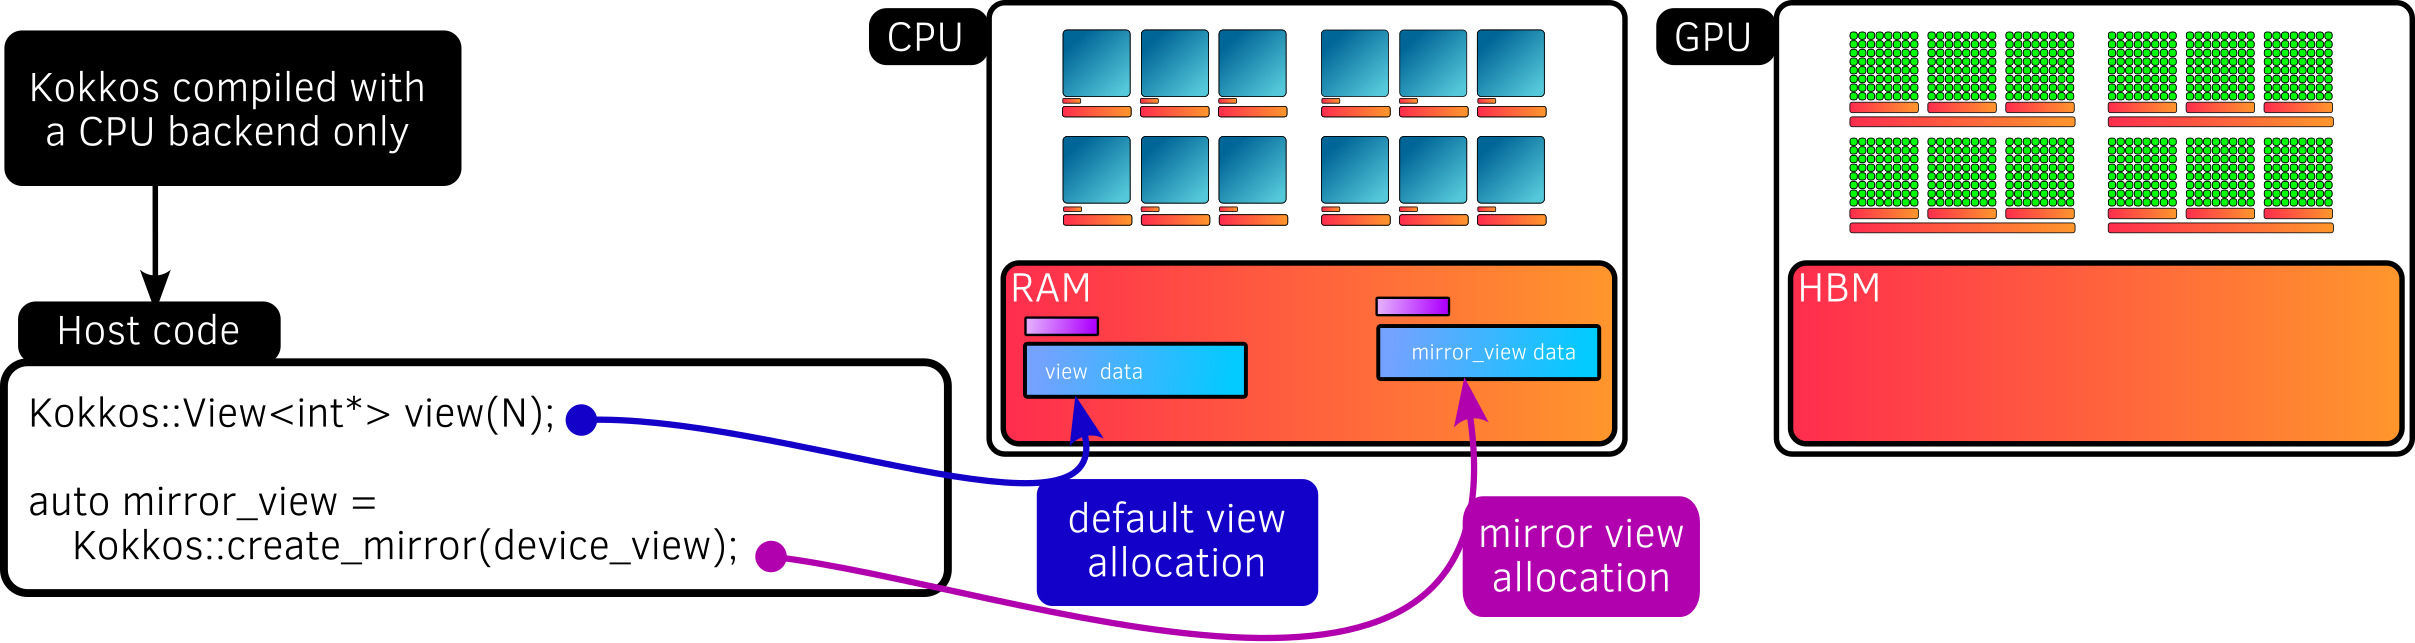
\includegraphics[width=0.9\textwidth]{host_mirror_view.png}
    \end{center}
    \begin{itemize}
        \item For portability reason, we always use a mirror view whether we compile with a CPU or GPU backend
        \item With a CPU backend only, the mirror view lives in the same memory space as the original view
    \end{itemize}

    \structure{Problem:} Memory is duplicated unnecessarily!
\end{frame}

% _____________________________________________________________________________

\begin{frame}[fragile]{All you need is a (different kind of) mirror}
    \begin{columns}
        \begin{column}{0.525\linewidth}
            \begin{minted}{C++}
                Kokkos::View<int**>
                    device_matrix("matrix", 10, 10);

                auto host_matrix =
                    Kokkos::create_mirror_view(
                        device_matrix
                    );
            \end{minted}
        \end{column}
        \begin{column}{0.475\linewidth}
            \begin{itemize}
                \item \texttt{create\_mirror\_view} creates a mirror without allocating memory if the mirror view lives in the same memory space as the original view
                \item In that case, the mirror view is a shallow copy of the original view (i.e. it targets the same data)
            \end{itemize}
        \end{column}
    \end{columns}
\end{frame}

% _____________________________________________________________________________

\begin{frame}{How to access data living on the Host from the Host?}
    \begin{center}
        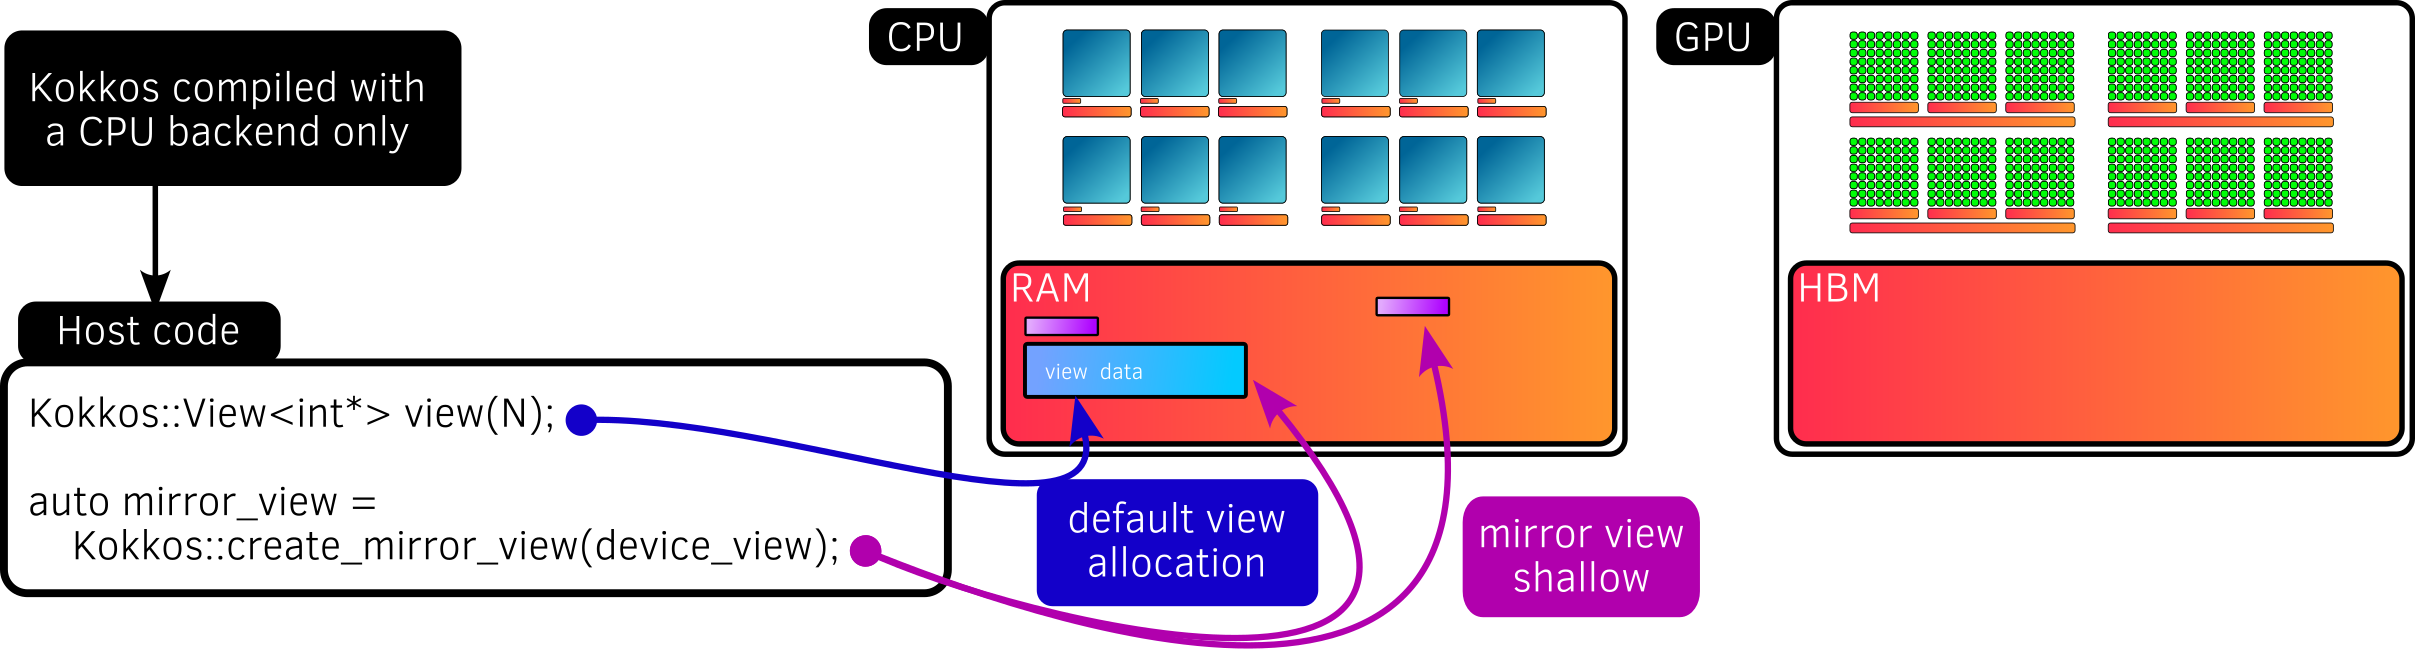
\includegraphics[width=0.9\textwidth]{host_create_mirror_view.png}
    \end{center}

    \structure{Solution:} Use \texttt{create\_mirror\_view}!
\end{frame}

% _____________________________________________________________________________

\begin{frame}[fragile]{Mirror functions wrap up}
    \begin{minted}{C++}
        auto mirror = Kokkos::create_mirror(view);
        auto mirror_view = Kokkos::create_mirror_view(view);
    \end{minted}
    \begin{center}
        \begin{tblr}[theme=kokkostable]{colspec=lll, row{2}={bg=lightmain}}
            & \SetCell[c=2]{l} Kokkos compiled on \\
            Mirror function & CPU backend & GPU backend \\
            \texttt{Kokkos::create\_mirror} & Allocate & Allocate \\
            \texttt{Kokkos::create\_mirror\_view} & No allocate & Allocate \\
        \end{tblr}
    \end{center}

    \structure{Problem:} How to transfer data, now?
\end{frame}

% _____________________________________________________________________________

\begin{frame}[fragile]{Deep copy data between memory spaces}
    \begin{columns}
        \begin{column}{0.6\linewidth}
            \begin{minted}{C++}
                Kokkos::View<int**>
                    device_matrix("matrix", Nx, Ny);

                auto host_matrix =
                    Kokkos::create_mirror(device_matrix);

                initialize(host_matrix);

                // from Host to Device
                Kokkos::deep_copy(
                    device_matrix,
                    host_matrix
                );
            \end{minted}
        \end{column}
        \begin{column}{0.4\linewidth}
            \begin{itemize}
                \item \texttt{deep\_copy} to copy data between views in different memory spaces
                \item Views must similar (shape, layout, etc.)
                \item If the destination view is a shallow copy of the source view (e.g. \texttt{create\_mirror\_view} on Host), the function does nothing (portability)
            \end{itemize}
        \end{column}
    \end{columns}
\end{frame}

% _____________________________________________________________________________

\begin{frame}{How to deep copy between the Host and the Device?}
    \begin{center}
        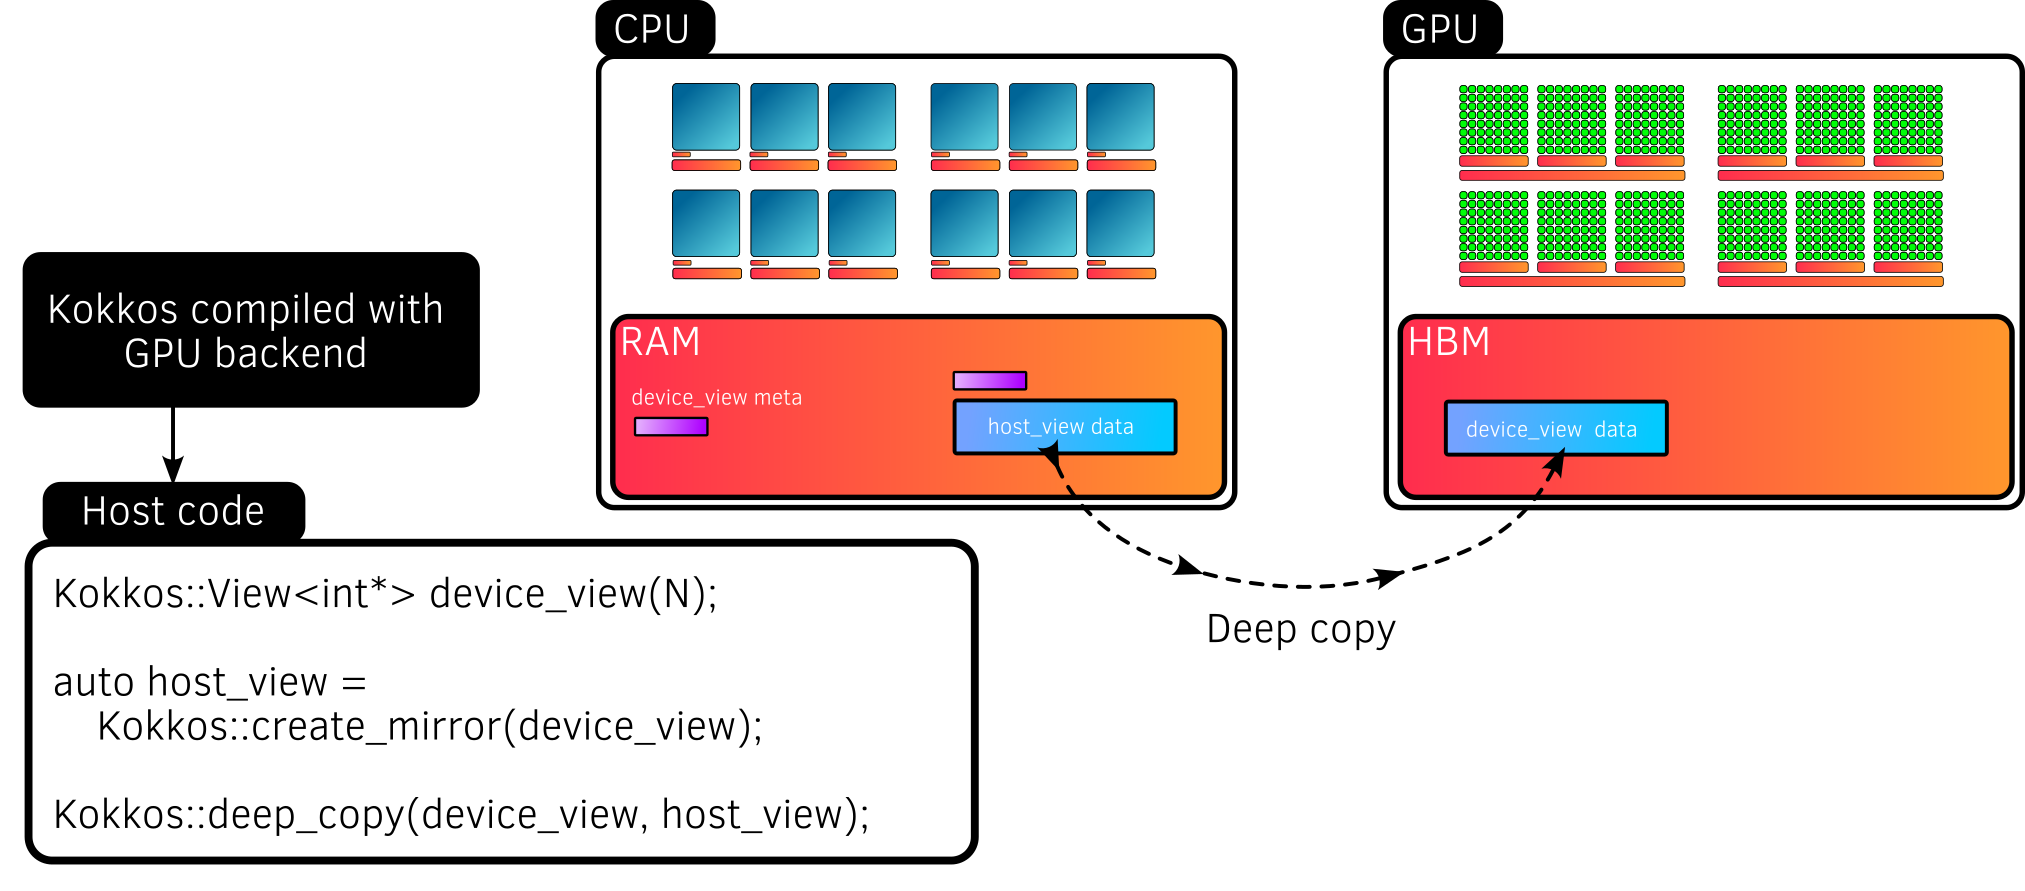
\includegraphics[width=0.9\textwidth]{host_device_deep_copy.png}
    \end{center}

    \structure{Solution:} With \texttt{deep\_copy}!
\end{frame}

% _____________________________________________________________________________

\begin{exerciseframe}{Exercise 3: Mirror Views and deep copy}
    \begin{columns}
        \begin{column}{0.5\linewidth}
            \begin{center}
                
\includegraphics[width=0.9\textwidth]{sleeping_otter.png}
            \end{center}

            Go to the exercise \githublink{\href{https://github.com/CExA-project/cexa-kokkos-tutorials/tree/main/exercises/03_deep_copy}{03\_deep\_copy}} and follow the instructions
        \end{column}
        \begin{column}{0.5\linewidth}
            \begin{block}{Goal of this exercise}
                \begin{itemize}
                    \item Create and manage a mirror view
                    \item Use the \texttt{deep\_copy} function
                    \item Observe the differences between the two mirror functions
                    \begin{itemize}
                        \item Timing
                        \item Memory (on Unixes only)
                    \end{itemize}
                \end{itemize}
            \end{block}
        \end{column}
    \end{columns}
\end{exerciseframe}

\begin{exerciseframe}{Exercise 3: Ruche environment}
    \begin{itemize}
        \item {\small \doclink{\url{https://github.com/CExA-project/kokkos-training-2025-barcelona}}}
        \item Environment for the hands-on
        \begin{minted}{sh}
            module load gcc/11.2.0/gcc-4.8.5 \
                        cmake/3.28.3/gcc-11.2.0 \
                        cuda/12.2.1/gcc-11.2.0
            export OMP_PROC_BIND=spread \
                   OMP_PLACES=threads
        \end{minted}
        \item Command to run on CPU
        \begin{minted}{sh}
            srun --partition cpu_short --cpus-per-task 20 --pty path/to/exe
        \end{minted}
        \item Command to run on GPU
        \begin{minted}{sh}
            srun --partition gpu --gres gpu:1 --pty path/to/exe
        \end{minted}
    \end{itemize}
\end{exerciseframe}

% _____________________________________________________________________________

\subsection{Parallel loops}

% _____________________________________________________________________________

\begin{frame}[fragile]{Anatomy of a loop}
    \begin{columns}
        \begin{column}{0.5\linewidth}
            \begin{minted}[texcomments]{C++}
                for (int i = 0; i < N; i++) {
                    A(i) = B(i) + C(i) * D(i);
                }
            \end{minted}
        \end{column}
        \begin{column}{0.5\linewidth}
            \begin{itemize}
                \item \mintinline{C++}{for} is the loop pattern (for, reduction, scan, graph)
                \item \mintinline{C++}{int i = 0; i < N; i++} is the execution policy
                \item \mintinline{C++}{A(i) = B(i) + C(i) * D(i)} is the kernel
                \begin{itemize}
                    \item No iteration order dependencies
                    \item No side effects
                \end{itemize}
            \end{itemize}
        \end{column}
    \end{columns}
\end{frame}

% _____________________________________________________________________________

\begin{frame}[fragile]{Comparison of Kokkos and OpenMP parallel loops}
    \begin{columns}[T]
        \begin{column}{0.5\linewidth}
            OpenMP version

            \begin{minted}{C++}
                #pragma omp parallel for
                for (int i = 0; i < N; i++) {
                    A(i) = B(i) + C(i) * D(i);
                }
            \end{minted}
            \begin{block}{Note}
                Only works on CPUs (need \texttt{target} directive for GPUs)
            \end{block}
        \end{column}
        \begin{column}{0.5\linewidth}
            Kokkos version

            \begin{minted}{C++}
                Kokkos::parallel_for(
                    "my_loop",
                    N,
                    KOKKOS_LAMBDA (int i) {
                        A(i) = B(i) + C(i) * D(i);
                    }
                );
            \end{minted}
            \begin{block}{Note}
                Works on CPUs and GPUs depending on the compiled backend
            \end{block}
        \end{column}
    \end{columns}
\end{frame}

% _____________________________________________________________________________

\begin{frame}[fragile]{Anatomy of a Kokkos parallel loop}
    \begin{columns}
        \begin{column}{0.5\linewidth}
            \begin{minted}{C++}
                Kokkos::parallel_for(
                    "my_loop",
                    N,
                    KOKKOS_LAMBDA (int i) {
                        A(i) = B(i) + C(i) * D(i);
                    }
                );
            \end{minted}
        \end{column}
        \begin{column}{0.5\linewidth}
            \begin{itemize}
                \item \mintinline{C++}{parallel_for} is the loop pattern
                \item \mintinline{C++}{"my_loop"} is the name of the loop (bonus for debugging!)
                \item \mintinline{C++}{N} and \mintinline{C++}{int i} is the execution policy (can't be simpler)
                \item \mintinline[breaklines]{C++}{KOKKOS_LAMBDA (int i) {/*...*/}} is the kernel
            \end{itemize}
        \end{column}
    \end{columns}

    \vspace{1em}

    \structure{Question:} What is this \texttt{KOKKOS\_LAMBDA} thingy?
\end{frame}

% _____________________________________________________________________________

\begin{frame}[fragile]{Notion of C++ lambdas}
    \begin{columns}
        \begin{column}{0.5\linewidth}
            \begin{minted}{C++}
                auto kernel =
                    KOKKOS_LAMBDA (int i) {
                        A(i) = B(i) + C(i) * D(i);
                    };
            \end{minted}
        \end{column}
        \begin{column}{0.5\linewidth}
            \begin{itemize}
                \item A lambda is a C++ anonymous function (i.e. a function as an object)
                \item It has explicit arguments (\mintinline{C++}{int i}) and captured objects (\texttt{A}, \texttt{B}, \texttt{C}, \texttt{D})
                \item \texttt{KOKKOS\_LAMBDA} is a macro that creates a lambda function with the correct capture for you (and a bit more)
                \item For beginners, no need to understand C++ lambdas to use Kokkos
            \end{itemize}
        \end{column}
    \end{columns}
\end{frame}

% _____________________________________________________________________________

\begin{frame}{Now, where is my parallel loop executed?}
    \begin{center}
        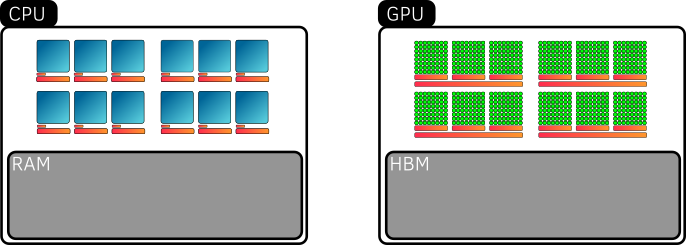
\includegraphics[width=0.8\linewidth]{execution_space.png}
    \end{center}
    \begin{itemize}
        \item Kokkos abstraction for where the loop is executed : \highlight{execution space}
        \item By default, parallel code (i.e. inside a \texttt{parallel\_*}) is executed
        \begin{itemize}
            \item By the Host if no GPU backend is available
            \item By the Device otherwise
        \end{itemize}
        \item What is not parallel code (the rest) is always executed by the Host
    \end{itemize}
\end{frame}

% _____________________________________________________________________________

\begin{frame}[fragile]{Asynchronous execution on GPU}
    \begin{columns}
        \begin{column}{0.5\linewidth}
            \begin{minted}{C++}
                // parallel loop on Device
                Kokkos::parallel_for(
                    "my_loop",
                    N,
                    KOKKOS_LAMBDA (int i) {
                        data(i) = ...
                    }
                );

                // Host code
                host_function(data);
            \end{minted}
        \end{column}
        \begin{column}{0.5\linewidth}
            \begin{itemize}
                \item With a GPU backend, the parallel loop is executed asynchronously on the GPU
                \item The loop is launched and the program continues
                \item Asynchronism is a complex concept for beginners, not covered in this talk
            \end{itemize}
        \end{column}
    \end{columns}

    \vspace{1em}
    \structure{Problem:} What if I need the results of the parallel loop in the host code?
\end{frame}

% _____________________________________________________________________________

\begin{frame}[fragile]{All you need is a fence}
    \begin{columns}
        \begin{column}{0.5\linewidth}
            \begin{minted}{C++}
                // parallel loop on Device
                Kokkos::parallel_for(
                    "my_loop",
                    N,
                    KOKKOS_LAMBDA (int i) {
                        data(i) = ...
                    }
                );

                Kokkos::fence("my_loop fence");

                // Host code
                host_function(data);
            \end{minted}
        \end{column}
        \begin{column}{0.5\linewidth}
            \begin{itemize}
                \item \texttt{fence} to wait for asynchronous work to be completed
                \item Equivalent to OpenMP \texttt{barrier} or to \texttt{MPI\_Wait}
            \end{itemize}
        \end{column}
    \end{columns}

    \vspace{1em}
    \structure{Solution:} With a fence
\end{frame}

% _____________________________________________________________________________

\begin{exerciseframe}{Exercise 4: My first parallel loop}
    \begin{columns}
        \begin{column}{0.5\linewidth}
            \begin{center}
                
\includegraphics[width=0.9\textwidth]{sleeping_otter.png}
            \end{center}

            Go to the exercise \githublink{\href{https://github.com/CExA-project/cexa-kokkos-tutorials/tree/main/exercises/04_parallel_loop}{04\_parallel\_loop}} and follow the instructions
        \end{column}
        \begin{column}{0.5\linewidth}
            \begin{block}{Goal of this exercise}
                \begin{itemize}
                    \item Write a simple parallel loop
                    \item Measure the difference of performance between CPU and GPU
                \end{itemize}
            \end{block}
        \end{column}
    \end{columns}
\end{exerciseframe}

\begin{exerciseframe}{Exercise 4: Ruche environment}
    \begin{itemize}
        \item {\small \doclink{\url{https://github.com/CExA-project/kokkos-training-2025-barcelona}}}
        \item Environment for the hands-on
        \begin{minted}{sh}
            module load gcc/11.2.0/gcc-4.8.5 \
                        cmake/3.28.3/gcc-11.2.0 \
                        cuda/12.2.1/gcc-11.2.0
            export OMP_PROC_BIND=spread \
                   OMP_PLACES=threads
        \end{minted}
        \item Command to run on CPU
        \begin{minted}{sh}
            srun --partition cpu_short --cpus-per-task 20 --pty path/to/exe
        \end{minted}
        \item Command to run on GPU
        \begin{minted}{sh}
            srun --partition gpu --gres gpu:1 --pty path/to/exe
        \end{minted}
    \end{itemize}
\end{exerciseframe}

% _____________________________________________________________________________

\subsection{Extending loop policies}

% _____________________________________________________________________________

\begin{frame}[fragile]{How to extend loop policies?}
    \begin{columns}
        \begin{column}{0.55\linewidth}
            \begin{minted}{C++}
                Kokkos::RangePolicy<ExecutionSpace>
                    policy(start_index, end_index);
            \end{minted}
        \end{column}
        \begin{column}{0.45\linewidth}
            \begin{itemize}
                \item Kokkos way to tell how a loop is executed: \highlight{execution policy}
                \item \texttt{RangePolicy} for single-dimensional loops
                \item \texttt{ExecutionSpace} for specifying where the loop is executed (defaults to \texttt{DefaultExecutionSpace})
                \item \texttt{start\_index} and \texttt{end\_index} are the beginning and the end (excluded) of the loop
            \end{itemize}
        \end{column}
    \end{columns}
\end{frame}

% _____________________________________________________________________________

\begin{frame}[fragile]{Loop policy shortcut}
    \begin{columns}
        \begin{column}{0.45\linewidth}
            Shortcut version\strut

            \begin{minted}{C++}
                Kokkos::parallel_for(
                    "my_loop",
                    N,


                    KOKKOS_LAMBDA (int i) {
                        /* ... */
                    }
                );
            \end{minted}
        \end{column}
        \begin{column}{0.55\linewidth}
            Explicit version (same)\strut

            \begin{minted}{C++}
                Kokkos::parallel_for(
                    "my_loop",
                    Kokkos::RangePolicy<
                        Kokkos::DefaultExecutionSpace
                    >(0, N),
                    KOKKOS_LAMBDA (int i) {
                        /* ... */
                    }
                );
            \end{minted}
        \end{column}
    \end{columns}
\end{frame}

% _____________________________________________________________________________

\begin{frame}{Execution space}
    \begin{itemize}
        \item Execution space to control where the loop is executed (CPU or GPU)
        \item Several ones available
        \item \texttt{Kokkos::DefaultExecutionSpace} and \texttt{Kokkos::DefaultHostExecutionSpace} are enough for beginners
        \item Using a backend-specific execution space is possible, but it breaks portability
    \end{itemize}
    \begin{center}
        \begin{tblr}[theme=kokkostable]{colspec=lll, row{2}={bg=lightmain}}
            & \SetCell[c=2]{l} Kokkos compiled on \\
            Execution space & CPU backend & GPU backend \\
            \texttt{Kokkos::DefaultExecutionSpace} & On CPU & On GPU \\
            \texttt{Kokkos::DefaultHostExecutionSpace} & On CPU & On CPU \\
        \end{tblr}
    \end{center}
\end{frame}

% _____________________________________________________________________________

\begin{frame}[fragile]{Relation between execution space and memory space}
    \begin{itemize}
        \item That relation makes sense (both on same hardware)
        \item \texttt{memory\_space} attribute to access the memory space associated with an execution space
        \item \texttt{HostSpace} for memory space of the default host execution space
    \end{itemize}
    \begin{center}
        % allow the table to overflow horizontally
        \makebox[\linewidth][c]{%
            \begin{tblr}[theme=kokkostable]{colspec=lll, row{2}={bg=lightmain}}
                & \SetCell[c=2]{l} Kokkos compiled on \\
                Memory space & CPU backend & GPU backend \\
                \texttt{Kokkos::DefaultExecutionSpace::memory\_space} & On CPU & On GPU \\
                \texttt{Kokkos::DefaultHostExecutionSpace::memory\_space} & On CPU & On CPU \\
            \end{tblr}%
        }
    \end{center}
\end{frame}

% _____________________________________________________________________________

\begin{frame}[fragile]{Anatomy of a nested loops}
    \begin{columns}
        \begin{column}{0.5\linewidth}
            \begin{minted}{C++}
                for (int i = 0; i < Nx; i++)
                    for (int j = 0; j < Ny; j++) {
                        A(i, j) = i + j;
                    }
            \end{minted}
        \end{column}
        \begin{column}{0.5\linewidth}
            \begin{itemize}
                \item 2 loop patterns
                \begin{itemize}
                    \item No extra code before/after the inner loop
                    \item Loops are collapsable (OpenMP \texttt{collapse})
                \end{itemize}
                \item 2 execution policies
                \begin{itemize}
                    \item No dependencies between them
                \end{itemize}
                \item 1 kernel
                \begin{itemize}
                    \item No iteration order dependencies
                    \item No side effects
                \end{itemize}
            \end{itemize}
        \end{column}
    \end{columns}
\end{frame}

% _____________________________________________________________________________

\begin{frame}[fragile]{How to have multidimensional loop policies?}
    \begin{columns}
        \begin{column}{0.6\linewidth}
            \begin{minted}{C++}
                Kokkos::MDRangePolicy<
                    ExecutionSpace,
                    Rank<n>
                > policy(
                    {start_index_0, ..., start_index_n},
                    {end_index_0, ..., end_index_n}
                );
            \end{minted}
        \end{column}
        \begin{column}{0.4\linewidth}
            \begin{itemize}
                \item \texttt{MDRangePolicy} for nested loops (with \emph{MD} for multidimensional)
                \item \texttt{Rank} template parameter to specify the dimension
                \item Max rank is 6
                \item \texttt{start\_index\_*} and \texttt{end\_index\_*} are the beginning and the end (excluded) of each loop
            \end{itemize}
        \end{column}
    \end{columns}
\end{frame}

% _____________________________________________________________________________

\begin{frame}[fragile]{Anatomy of a Kokkos nested loop}
    \begin{columns}
        \begin{column}{0.6\linewidth}
            \begin{minted}{C++}
                Kokkos::parallel_for(
                    "my_loop",
                    Kokkos::MDRangePolicy<
                        ExecutionSpace,
                        Kokkos::Rank<2>
                    >({0, 0}, {Nx, Ny}),
                    KOKKOS_LAMBDA (int i, int j) {
                        A(i, j) = i + j;
                    }
                );
            \end{minted}
        \end{column}
        \begin{column}{0.4\linewidth}
            \begin{itemize}
                \item Still 1 \texttt{parallel\_for}
                \item No shortcut version!
                \item Kernel has 2 arguments
            \end{itemize}
        \end{column}
    \end{columns}
\end{frame}

% _____________________________________________________________________________

\subsection[Parallel reduction]{Parallel reduction}

% _____________________________________________________________________________

\begin{frame}[fragile]{Anatomy of a reduction loop}
    \begin{columns}
        \begin{column}{0.5\linewidth}
            \begin{minted}[texcomments]{C++}
                double result = 0;

                for (int i = 0; i < N; i++) {
                    result += A(i);
                }
            \end{minted}
        \end{column}
        \begin{column}{0.5\linewidth}
            \begin{itemize}
                \item One scalar variable collects something for each iteration (sum, max, min, etc.)
                \item Same constraints as before
                \item Horrible truth: \texttt{result} value \highlight{depends} on iteration order!
            \end{itemize}
        \end{column}
    \end{columns}
\end{frame}

% _____________________________________________________________________________

\begin{frame}[fragile]{Anatomy of a Kokkos parallel reduction loop}
    \begin{columns}
        \begin{column}{0.5\linewidth}
            \begin{minted}{C++}
                // no initialization needed,
                // handled by parallel reduce
                double result;

                Kokkos::parallel_reduce(
                    "my_reduction",
                    N,
                    KOKKOS_LAMBDA (
                        int i,
                        double& local_result
                    ) {
                        local_result += i;
                    },
                    Kokkos::Sum<double>(result)
                );
            \end{minted}
        \end{column}
        \begin{column}{0.5\linewidth}
            \begin{itemize}
                \item \texttt{parallel\_reduce} to perform reductions
                \item Works like \texttt{parallel\_for} (e.g. execution space)
                \item Reducer object (here \texttt{Sum}), templated with the result type
                \item Extra last argument to the kernel: a reference to the local result
            \end{itemize}
        \end{column}
    \end{columns}
\end{frame}

% _____________________________________________________________________________

\begin{frame}{About reducers}
    \begin{itemize}
        \item Kokkos provides reducers for the most common operations:
        \begin{itemize}
            \item \texttt{Kokkos::Sum}: Sum of the elements
            \item \texttt{Kokkos::Max}: and \texttt{Kokkos::Min}: Maximum and minimum element
            \item \texttt{Kokkos::Prod}: Product of the elements
            \item \texttt{Kokkos::MaxLoc} and \texttt{Kokkos::MinLoc}: Maximum and minimum element with their index
            \item More \doclink{\href{https://kokkos.org/kokkos-core-wiki/ProgrammingGuide/Custom-Reductions-Built-In-Reducers.html}{in the doc}}
        \end{itemize}
        \item You can also create your own reducer, not covered in this talk
    \end{itemize}
\end{frame}

% _____________________________________________________________________________

\begin{frame}[fragile]{Sum reduction example}
    \begin{minted}{C++}
        double result;
        Kokkos::parallel_reduce(
            "my_reduction",
            N,
            KOKKOS_LAMBDA (int i, double& local_result) {
                local_result += A(i);
            },
            result // shortcut for sum
        );
    \end{minted}
\end{frame}

% _____________________________________________________________________________

\begin{frame}[fragile]{Max reduction example}
    \begin{minted}{C++}
        double max_value;
        Kokkos::parallel_reduce(
            "my_reduction",
            N,
            KOKKOS_LAMBDA (int i, double& local_max_value) {
                local_max_value = Kokkos::max(A(i), local_max_value);
            },
            Kokkos::Max<double>(max_value)
        );
    \end{minted}

    \structure{Note:} Notice that mathematical operators are in the \texttt{Kokkos} namespace
\end{frame}

% _____________________________________________________________________________

\begin{frame}[fragile]{Min and index reduction example}
    \begin{minted}{C++}
        // Use a structure containing val and loc variables
        using minloc_type = Kokkos::MinLoc<double, int>::value_type;

        minloc_type minloc;
        Kokkos::parallel_reduce(
            "MinLocReduce",
            N,
            KOKKOS_LAMBDA (int i, minloc_type& local_minloc_value) {
                if (A(i) < local_minloc_value.val) {
                    local_minloc_value.val = A(i);
                    local_minloc_value.loc = i;
                }
            },
            Kokkos::MinLoc<double, int>(minloc)
        );
    \end{minted}
\end{frame}

% _____________________________________________________________________________

\begin{exerciseframe}{Exercise 5: Parallel Reduction}
    \begin{columns}
        \begin{column}{0.5\linewidth}
            \begin{center}
                
\includegraphics[width=0.9\textwidth]{sleeping_otter.png}
            \end{center}

            Go to the exercise \githublink{\href{https://github.com/CExA-project/cexa-kokkos-tutorials/tree/main/exercises/05_parallel_reduce}{05\_parallel\_reduce}} and follow the instructions
        \end{column}
        \begin{column}{0.5\linewidth}
            \begin{block}{Goal of this exercise}
                \begin{itemize}
                    \item Perform a parallel reduction
                    \item Measure the difference of performance between CPU and GPU
                \end{itemize}
            \end{block}
        \end{column}
    \end{columns}
\end{exerciseframe}

\begin{exerciseframe}{Exercise 5: Ruche environment}
    \begin{itemize}
        \item {\small \doclink{\url{https://github.com/CExA-project/kokkos-training-2025-barcelona}}}
        \item Environment for the hands-on
        \begin{minted}{sh}
            module load gcc/11.2.0/gcc-4.8.5 \
                        cmake/3.28.3/gcc-11.2.0 \
                        cuda/12.2.1/gcc-11.2.0
            export OMP_PROC_BIND=spread \
                   OMP_PLACES=threads
        \end{minted}
        \item Command to run on CPU
        \begin{minted}{sh}
            srun --partition cpu_short --cpus-per-task 20 --pty path/to/exe
        \end{minted}
        \item Command to run on GPU
        \begin{minted}{sh}
            srun --partition gpu --gres gpu:1 --pty path/to/exe
        \end{minted}
    \end{itemize}
\end{exerciseframe}

% _____________________________________________________________________________

\section[Conclusion]{Conclusion}

% _____________________________________________________________________________

\begin{frame}{Conclusion}
    Congratulation, you have learned the basics of Kokkos!

    \begin{itemize}
        \item How to compile Kokkos
        \item How to create and manage a simple View
        \item How to use mirror Views and deep copy
        \item How to write a parallel loop
        \item How to extend the loop policy
        \item How to use nested parallel loops
        \item How to write a parallel reduction
    \end{itemize}
\end{frame}

\end{document}
